\documentclass[11pt,letterpaper]{article}
\synctex=1

\usepackage[utf8]{inputenc}
\usepackage[T1]{fontenc}
\usepackage[spanish,es-tabla,es-nodecimaldot]{babel}
\usepackage{lmodern}
\usepackage{geometry}
\geometry{margin=2.15cm, top=2.0cm, bottom=2.1cm}

\usepackage{amsmath,amssymb}
\usepackage{graphicx}
\usepackage{booktabs}
\usepackage{caption}
\usepackage{float}
\usepackage{hyperref}
\usepackage{titlesec}
\usepackage{parskip}

\hypersetup{
    hidelinks,
    pdftitle={Examen 2 - Parte Práctica: Órbitas Estelares en Disco de Kuzmin y Halo de Miyamoto-Nagai},
    pdfauthor={Bryan Camilo Restrepo Arcila}
}

\titleformat{\section}{\large\bfseries}{\thesection.}{0.5em}{}
\titleformat{\subsection}{\normalsize\bfseries}{\thesubsection}{0.5em}{}
\captionsetup{font=small, labelfont=bf, margin=0.3cm}

\graphicspath{{../figures/}}

\begin{document}

% =============================================================================
% Encabezado del informe
% =============================================================================
\noindent{\Large\bfseries Dinámica de Órbitas Estelares en un Disco de Kuzmin y Efecto de un Halo Oblato de Materia Oscura}

\vspace{6pt}
\noindent
\textbf{Curso:} Astrofísica Galáctica y Extragaláctica (Examen 2, Parte Práctica)\\
\textbf{Estudiante:} Bryan Camilo Restrepo Arcila\\
\textbf{Profesor:} Juan Carlos Muñoz Cuartas\\
Instituto de Física, Universidad de Antioquia\\
Noviembre de 2026

\vspace{4pt}
\hrule height 0.6pt
\vspace{8pt}

% =============================================================================
% Contexto, modelo de galaxia y sistema de unidades
% =============================================================================
\section*{Planteamiento del modelo y elección de parámetros}

El potencial de Kuzmin (Binney \& Tremaine, 2008, \S 2.3.1, Ec.~2.68a, p.~72) es:
\begin{equation}
    \Phi_K(R, z) = -\frac{G M_d}{\sqrt{R^2 + (a_d + |z|)^2}}, \qquad a_d > 0,
    \label{eq:phi_kuzmin}
\end{equation}
donde $(R, \phi, z)$ son coordenadas cilíndricas, $M_d$ es la masa total del disco y $a_d$ es su longitud de escala radial. 
Este es el potencial que describe un disco infinitamente delgado.

Mediante el teorema de Gauss en una caja delgada que encierra el plano $z = 0$ (Binney \& Tremaine, 2008, \S 2.3.1, Ec.~2.68b, p.~72; usando la Ec.~2.12, p.~58), este potencial corresponde a la densidad superficial
\begin{equation}
    \Sigma_K(R) = \frac{a_d M_d}{2\pi (R^2 + a_d^2)^{3/2}},
    \label{eq:sigma_kuzmin}
\end{equation}
cuya masa encerrada hasta un radio $R$ se obtiene integrando $2\pi R'\Sigma_K(R')\,\mathrm{d}R'$ desde $0$ hasta $R$. Haciendo la sustitución $u = R'^2 + a_d^2$, con $\mathrm{d}u = 2R'\,\mathrm{d}R'$ (es decir, $R'\,\mathrm{d}R' = \tfrac{1}{2}\,\mathrm{d}u$) y límites $u(0) = a_d^2$ y $u(R) = R^2 + a_d^2$:
\begin{align}
    M_d(<R) &= \int_0^R 2\pi R'\Sigma_K(R')\,\mathrm{d}R'
    = a_d M_d \int_0^R \frac{R'\,\mathrm{d}R'}{(R'^2 + a_d^2)^{3/2}}
    = \frac{a_d M_d}{2} \int_{a_d^2}^{R^2 + a_d^2} u^{-3/2}\,\mathrm{d}u \nonumber \\
    &= \frac{a_d M_d}{2}\left[-2 u^{-1/2}\right]_{a_d^2}^{R^2 + a_d^2}
    = a_d M_d\left(\frac{1}{a_d} - \frac{1}{\sqrt{R^2 + a_d^2}}\right)
    = M_d\left(1 - \frac{a_d}{\sqrt{R^2 + a_d^2}}\right).
\end{align}


\paragraph{Parámetros del disco.}
\mbox{}\\[0.4em]
El último dígito de mi cédula es el 5, la masa del disco entonces es de:
\begin{equation}
    M_d = 5 \times 10^{11}\,M_\odot = 50\,M_u.
\end{equation}
Según Binney \& Tremaine (2008, Tabla~2.3, p.~113), el disco de la Vía Láctea tiene una masa de $\sim 5\times 10^{10}\,M_\odot$, longitud de escala $R_d \approx 2$--$3.2\,\mathrm{kpc}$ y velocidad circular cercana a $220\,\mathrm{km\,s^{-1}}$.

En el modelo de Kuzmin, maximizar la velocidad circular $v_c^2 = R\,\partial\Phi_K/\partial R|_{z=0}$ respecto a $R$ (Sección~1.1) da un máximo en $R_{\mathrm{max}} = \sqrt{2}\,a_d$ con valor $v_{c,\max} = \sqrt{2GM_d/(3\sqrt{3}\,a_d)}$. Como aquí la masa del disco es diez veces mayor ($5\times 10^{11}\,M_\odot$), mantener una escala pequeña como $a_d = 2$--$3\,\mathrm{kpc}$ daría $v_{c,\max} > 520\,\mathrm{km\,s^{-1}}$, más del doble que en la Vía Láctea. Por tanto, se aumenta $a_d$ para mantener velocidades en el mismo orden de magnitud, así que:
\begin{equation}
    a_d = 8.0\,\mathrm{kpc}.
\end{equation}
En el sistema de unidades recomendado ($M_u = 10^{10}\,M_\odot$, $L_u = 1\,\mathrm{kpc}$ y $G = 43007.1\,\mathrm{kpc\,km^2\,s^{-2}\,M_u^{-1}}$), las velocidades salen directamente en $\mathrm{km\,s^{-1}}$ y la unidad de tiempo coherente es $t_u = L_u/V_u = 1\,\mathrm{kpc}/(1\,\mathrm{km\,s^{-1}}) = 3.0857 \times 10^{16}\,\mathrm{s} \approx 0.978\,\mathrm{Gyr}$. Con estos parámetros, el disco tiene radio de media masa $R_{1/2} = \sqrt{3}\,a_d \approx 13.9\,\mathrm{kpc}$, densidad superficial central $\Sigma_K(0) = 1243\,M_\odot\,\mathrm{pc}^{-2}$ y velocidad circular máxima $v_{c,\max} = 321.7\,\mathrm{km\,s^{-1}}$ en $R_{\mathrm{max}} \approx 11.3\,\mathrm{kpc}$ (Figura~\ref{fig:kuzmin_structure}).

\begin{figure}[H]
    \centering
    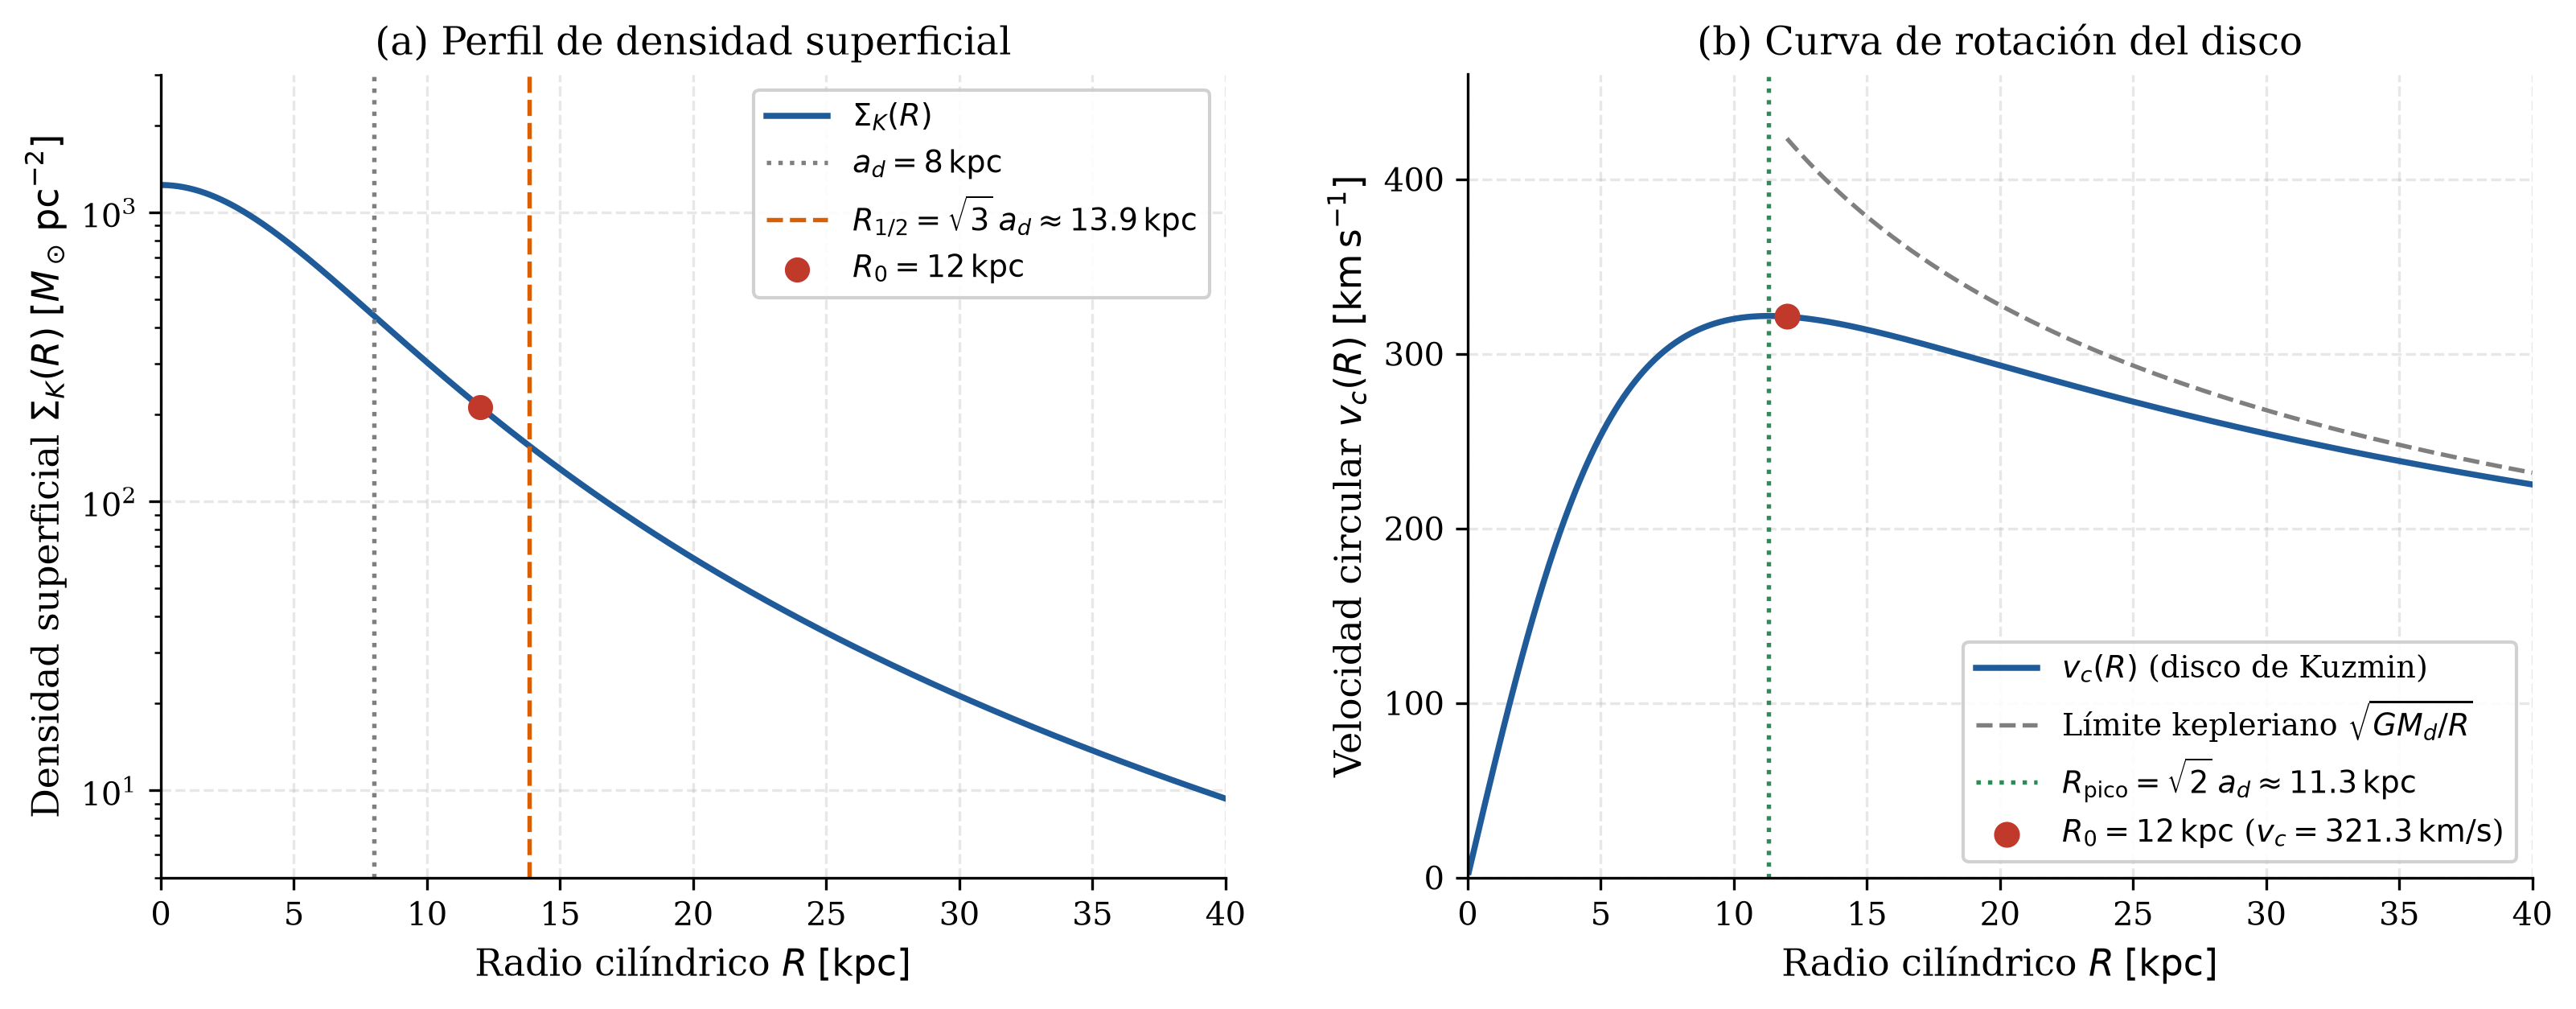
\includegraphics[width=0.98\textwidth]{fig1_kuzmin_structure.png}
    \caption{Perfil del disco de Kuzmin ($M_d = 5\times 10^{11}\,M_\odot$, $a_d = 8\,\mathrm{kpc}$). (a) Densidad superficial $\Sigma_K(R)$, escala $a_d$, radio de media masa $R_{1/2}$ y radio de estudio $R_0 = 12\,\mathrm{kpc}$. (b) Curva de rotación $v_c(R)$ comparada con el límite kepleriano $\sqrt{GM_d/R}$.}
    \label{fig:kuzmin_structure}
\end{figure}

% =============================================================================
% Numeral 1: Predicciones analíticas
% =============================================================================
\section{Predicciones analíticas para órbitas levemente fuera del equilibrio}

El potencial de Kuzmin, $\Phi_K(R, z) = -GM_d / \sqrt{R^2 + (a_d + |z|)^2}$, es estacionario y con simetría axial (no depende de $t$ ni de $\phi$). Siguiendo a Binney \& Tremaine (2008, \S 3.1, p.~143 y \S 3.1.1, p.~156), como la trayectoria gravitacional no depende de la masa de la estrella se trabaja por unidad de masa; por tanto, se conservan la energía específica (energía por unidad de masa) $E$ y el momento angular vertical por unidad de masa $L_z$:
\begin{equation}
    E = \frac{1}{2}\left(\dot{R}^2 + R^2\dot{\phi}^2 + \dot{z}^2\right) + \Phi_K(R, z),
    \qquad
    L_z = R^2\dot{\phi}.
\end{equation}

Para describir el movimiento en el plano meridional $(R, z)$, se parte del lagrangiano por unidad de masa en coordenadas cilíndricas:
\begin{equation}
    \mathcal{L}(R, z, \dot{R}, \dot{\phi}, \dot{z})
    = \frac{1}{2}\left(\dot{R}^2 + R^2\dot{\phi}^2 + \dot{z}^2\right) - \Phi_K(R, z).
\end{equation}
Al aplicar las ecuaciones de Euler-Lagrange, $\frac{\mathrm{d}}{\mathrm{d}t}\!\left(\frac{\partial \mathcal{L}}{\partial \dot{q}_i}\right) - \frac{\partial \mathcal{L}}{\partial q_i} = 0$, a cada coordenada:
\begin{itemize}
    \item Para $\phi$: como $\partial\mathcal{L}/\partial\phi = 0$, entonces $\frac{\mathrm{d}}{\mathrm{d}t}(R^2\dot{\phi}) = 0$, lo que confirma la conservación de $L_z = R^2\dot{\phi}$ y permite escribir $\dot{\phi} = L_z/R^2$.
    \item Para $R$ y $z$: las ecuaciones de movimiento resultan
    \begin{equation}
        \ddot{R} - R\dot{\phi}^2 = -\frac{\partial\Phi_K}{\partial R},
        \qquad
        \ddot{z} = -\frac{\partial\Phi_K}{\partial z}.
    \end{equation}
\end{itemize}
Sustituyendo $\dot{\phi} = L_z/R^2$ en la ecuación radial y reescribiendo el término centrífugo como una derivada respecto a $R$:
\begin{equation}
    \ddot{R} = -\frac{\partial\Phi_K}{\partial R} + \frac{L_z^2}{R^3}
    = -\frac{\partial}{\partial R}\!\left(\Phi_K(R, z) + \frac{L_z^2}{2R^2}\right).
\end{equation}
Como el término $L_z^2/(2R^2)$ no depende de $z$, su derivada respecto a $z$ es nula. Por tanto, definiendo el potencial efectivo (Binney \& Tremaine, 2008, \S 3.2.1):
\begin{equation}
    \boxed{\Phi_{\mathrm{eff}}(R, z) \equiv \Phi_K(R, z) + \frac{L_z^2}{2R^2}},
    \label{eq:phi_eff}
\end{equation}
el movimiento en el plano meridional $(R, z)$ queda gobernado directamente por
\begin{equation}
    \ddot{R} = -\frac{\partial\Phi_{\mathrm{eff}}}{\partial R},
    \qquad
    \ddot{z} = -\frac{\partial\Phi_{\mathrm{eff}}}{\partial z} = -\frac{\partial\Phi_K}{\partial z}.
\end{equation}

\subsection{Frecuencia de epiciclo radial \texorpdfstring{$\kappa(R)$}{kappa(R)}}

Una órbita circular de equilibrio en el plano $z = 0$ ocurre en el radio guía $R_g$ donde $(\partial\Phi_{\mathrm{eff}}/\partial R)_{R_g,0} = 0$. Para $\Phi_K(R, 0) = -GM_d (R^2 + a_d^2)^{-1/2}$:
\begin{equation}
    \left.\frac{\partial \Phi_K}{\partial R}\right|_{z=0}
    = -GM_d\left(-\frac{1}{2}\right)(R^2 + a_d^2)^{-3/2}(2R)
    = \frac{GM_d R}{(R^2 + a_d^2)^{3/2}}.
\end{equation}
De la condición de equilibrio $\left.\partial\Phi_{\mathrm{eff}}/\partial R\right|_{z=0} = 0$ con $\Phi_{\mathrm{eff}}(R, 0) = \Phi_K(R, 0) + L_z^2/(2R^2)$, y usando que en una órbita circular de velocidad tangencial $v_c = R\dot{\phi}$ el momento angular específico es $L_z = R^2\dot{\phi} = R v_c$ (de modo que $L_z^2/R^3 = v_c^2/R$), entonces:
\begin{equation}
    \left.\frac{\partial \Phi_K}{\partial R}\right|_{z=0} - \frac{L_z^2}{R^3} = 0
    \qquad \Longrightarrow \qquad
    \frac{v_c^2}{R} = \frac{L_z^2}{R^3} = \left.\frac{\partial \Phi_K}{\partial R}\right|_{z=0}.
\end{equation}
Despejando entonces $v_c(R)$ y la frecuencia angular circular $\Omega(R) = v_c(R)/R$:
\begin{gather}
    v_c(R) = \sqrt{R\left.\frac{\partial \Phi_K}{\partial R}\right|_{z=0}},
    \qquad
    \Omega(R) = \frac{v_c(R)}{R}, \nonumber \\[4pt]
    \boxed{v_c(R) = \sqrt{\frac{G M_d R^2}{(R^2 + a_d^2)^{3/2}}}}, \qquad
    \boxed{\Omega(R) = \sqrt{\frac{G M_d}{(R^2 + a_d^2)^{3/2}}}}.
    \label{eq:vc_omega}
\end{gather}

En la aproximación epicíclica, para un desplazamiento radial pequeño $x \equiv R - R_g$ ($|x| \ll R_g$) a $L_z$ constante, expandiendo el potencial efectivo en series de Taylor alrededor de $R_g$:
\begin{align}
    \Phi_{\mathrm{eff}}(R_g + x, 0)
    &\approx \Phi_{\mathrm{eff}}(R_g, 0)
    + \underbrace{
        \left(
            \frac{\partial \Phi_{\mathrm{eff}}}{\partial R}
        \right)_{R_g,\,0}
        x
    }_{\substack{=\,0 \\[1pt] (\partial_R\Phi_{\mathrm{eff}})_{R_g}=0}}
    + \frac{1}{2}
    \left(
        \frac{\partial^2 \Phi_{\mathrm{eff}}}{\partial R^2}
    \right)_{R_g,\,0}
    x^2 \nonumber \\
    &\approx \Phi_{\mathrm{eff}}(R_g, 0)
    + \frac{1}{2}
    \left(
        \frac{\partial^2 \Phi_{\mathrm{eff}}}{\partial R^2}
    \right)_{R_g,\,0}
    x^2.
    \label{eq:phi_eff_expansion}
\end{align}
Como $R(t) = R_g + x(t)$ con $R_g$ constante, se cumple $\ddot{R} = \ddot{x}$ y $\partial/\partial R = \partial/\partial x$. Al sustituir esta expansión en la ecuación radial $\ddot{R} = -\partial\Phi_{\mathrm{eff}}/\partial R$ y derivar respecto a $x$ (recordando que $\Phi_{\mathrm{eff}}(R_g, 0)$ y $(\partial^2\Phi_{\mathrm{eff}}/\partial R^2)_{R_g,\,0}$ son constantes evaluadas en $R_g$):
\begin{equation}
    \ddot{x} = -\frac{\partial \Phi_{\mathrm{eff}}}{\partial x}
    \approx -\frac{\partial}{\partial x}\!\left[
        \Phi_{\mathrm{eff}}(R_g, 0)
        + \frac{1}{2}\left(\frac{\partial^2 \Phi_{\mathrm{eff}}}{\partial R^2}\right)_{R_g,\,0} x^2
    \right]
    = -\left(\frac{\partial^2 \Phi_{\mathrm{eff}}}{\partial R^2}\right)_{R_g,\,0} x.
\end{equation}
Esta ecuación tiene exactamente la forma de un oscilador armónico simple $\ddot{x} = -\kappa^2 x$ (es decir, $\ddot{x} + \kappa^2 x = 0$), donde la frecuencia de epiciclo $\kappa$ está dada por (evaluando en un radio arbitrario $R$ y usando $L_z^2 = R^3\,\partial\Phi_K/\partial R|_{z=0} = R^4\Omega^2$):
\begin{align}
    \kappa^2(R) &= \left.\frac{\partial^2 \Phi_{\mathrm{eff}}}{\partial R^2}\right|_{R,0}
    = \frac{\partial^2}{\partial R^2}\!\left[\Phi_K(R, 0) + \frac{L_z^2}{2R^2}\right]
    = \left.\frac{\partial^2 \Phi_K}{\partial R^2}\right|_{z=0} + \frac{3 L_z^2}{R^4} \nonumber \\
    &= \left.\frac{\partial^2 \Phi_K}{\partial R^2}\right|_{z=0} + \frac{3}{R}\left.\frac{\partial \Phi_K}{\partial R}\right|_{z=0}
    = R\frac{\mathrm{d}\Omega^2}{\mathrm{d}R} + 4\Omega^2.
    \label{eq:kappa_def}
\end{align}
Recordando que anteriormente se obtuvo la primera derivada radial en el plano $z = 0$, $\left.\partial\Phi_K/\partial R\right|_{z=0} = GM_d R/(R^2 + a_d^2)^{3/2}$, al derivar una segunda vez respecto a $R$ resulta:
\begin{align}
    \left.\frac{\partial^2 \Phi_K}{\partial R^2}\right|_{z=0}
    &= \frac{\partial}{\partial R}\!\left[\frac{GM_d R}{(R^2 + a_d^2)^{3/2}}\right]
    = GM_d\,\frac{(R^2 + a_d^2)^{3/2} - 3R^2(R^2 + a_d^2)^{1/2}}{(R^2 + a_d^2)^3} \nonumber \\
    &= \frac{GM_d\,(a_d^2 - 2R^2)}{(R^2 + a_d^2)^{5/2}}.
\end{align}
Sustituyendo ambas derivadas en $\kappa^2(R) = \left.\partial^2\Phi_K/\partial R^2\right|_{z=0} + \frac{3}{R}\left.\partial\Phi_K/\partial R\right|_{z=0}$, se obtiene entonces la expresión exacta de $\kappa(R)$:
\begin{gather}
    \kappa^2(R) = \frac{GM_d\,(a_d^2 - 2R^2)}{(R^2 + a_d^2)^{5/2}} + \frac{3}{R}\,\frac{GM_d R}{(R^2 + a_d^2)^{3/2}}
    = \frac{GM_d\,(a_d^2 - 2R^2) + 3GM_d(R^2 + a_d^2)}{(R^2 + a_d^2)^{5/2}}, \nonumber \\[4pt]
    \boxed{\kappa^2(R) = \frac{GM_d\,(R^2 + 4a_d^2)}{(R^2 + a_d^2)^{5/2}}}.
    \label{eq:kappa_kuzmin}
\end{gather}
Dividiendo $\kappa^2(R)$ entre $\Omega^2(R) = GM_d/(R^2 + a_d^2)^{3/2}$ se obtiene la razón adimensional:
\begin{gather}
    \frac{\kappa(R)}{\Omega(R)} = \sqrt{\frac{R^2 + 4a_d^2}{R^2 + a_d^2}}, \nonumber \\[4pt]
    \boxed{\frac{\kappa(R)}{\Omega(R)} = \sqrt{1 + \frac{3a_d^2}{R^2 + a_d^2}}}.
    \label{eq:kappa_over_omega}
\end{gather}

\subsection{Frecuencia vertical \texorpdfstring{$\nu(R)$}{nu(R)}}

Para analizar ahora el movimiento en la dirección vertical, en un potencial suave y simétrico respecto al plano $z = 0$ (Binney \& Tremaine, 2008, \S 3.2.3), la expansión de Taylor alrededor de $z = 0$ es:
\begin{align}
    \Phi(R, z)
    &\approx \Phi(R, 0)
    + \underbrace{\left(\frac{\partial \Phi}{\partial z}\right)_{R,\,0} z}_{=\,0}
    + \frac{1}{2}\left(\frac{\partial^2 \Phi}{\partial z^2}\right)_{R,\,0} z^2 \nonumber \\
    &\approx \Phi(R, 0)
    + \frac{1}{2}\left(\frac{\partial^2 \Phi}{\partial z^2}\right)_{R,\,0} z^2.
\end{align}
Sustituyendo esta expansión en la ecuación vertical $\ddot{z} = -\partial\Phi/\partial z$, resulta un oscilador armónico simple:
\begin{equation}
    \ddot{z} \approx -\left(\frac{\partial^2 \Phi}{\partial z^2}\right)_{R,\,0} z = -\nu^2 z,
    \qquad \text{con} \qquad
    \nu^2(R) = \left.\frac{\partial^2 \Phi}{\partial z^2}\right|_{R,\,0}.
\end{equation}

Evaluando ahora estas derivadas para el potencial de Kuzmin $\Phi_K(R, z) = -GM_d\,[R^2 + (a_d + |z|)^2]^{-1/2}$, para $z \neq 0$ (usando $\mathrm{d}|z|/\mathrm{d}z = \operatorname{sgn}(z)$) la fuerza vertical resulta:
\begin{align}
    F_z(R, z) &= -\frac{\partial \Phi_K}{\partial z}
    = GM_d\left(-\frac{1}{2}\right)\left[R^2 + (a_d + |z|)^2\right]^{-3/2} \cdot 2(a_d + |z|)\,\operatorname{sgn}(z) \nonumber \\
    &= -\frac{GM_d\,(a_d + |z|)\,\operatorname{sgn}(z)}{\left[R^2 + (a_d + |z|)^2\right]^{3/2}}.
    \label{eq:Fz_kuzmin}
\end{align}
Recordando la densidad superficial del disco, $\Sigma_K(R) = a_d M_d / [2\pi(R^2 + a_d^2)^{3/2}]$, al evaluar los límites laterales de $F_z(R, z)$ por encima ($z \to 0^+$) y por debajo ($z \to 0^-$) del plano se obtiene:
\begin{align}
    \lim_{z \to 0^+} F_z(R, z) &= -\frac{GM_d a_d}{(R^2 + a_d^2)^{3/2}} = -2\pi G \Sigma_K(R), \nonumber \\
    \lim_{z \to 0^-} F_z(R, z) &= +\frac{GM_d a_d}{(R^2 + a_d^2)^{3/2}} = +2\pi G \Sigma_K(R).
    \label{eq:Fz_jump}
\end{align}
En una función continua ambos límites coincidirían y su diferencia sería nula; aquí, en cambio, al restar la fuerza justo debajo y justo encima del plano resulta un salto finito:
\begin{equation}
    \Delta F_z \equiv \lim_{z \to 0^-} F_z(R, z) - \lim_{z \to 0^+} F_z(R, z) = 4\pi G \Sigma_K(R) \neq 0,
\end{equation}
Al derivar una segunda vez respecto a $z$, esta discontinuidad produce una delta de Dirac en $z = 0$:
\begin{equation}
    \frac{\partial^2 \Phi_K}{\partial z^2} = 4\pi G \Sigma_K(R)\,\delta(z) + \frac{GM_d\left[R^2 - 2(a_d + |z|)^2\right]}{\left[R^2 + (a_d + |z|)^2\right]^{5/2}}.
    \label{eq:d2phi_dz2}
\end{equation}
De aquí se puede entender que en el disco de Kuzmin exacto la frecuencia armónica estándar $\nu^2 = (\partial^2\Phi_K/\partial z^2)_{R,\,0}$ diverge en $z = 0$; por tanto, la aproximación armónica cuadrática no es aplicable. Evaluar únicamente el segundo término en $z \to 0^+$ tampoco es válido, pues $R^2 - 2a_d^2$ es incluso negativo para $R < \sqrt{2}\,a_d$.

Este resultado coincide con interpretar el disco de Kuzmin como el límite $b \to 0$ del potencial de Miyamoto-Nagai (Binney \& Tremaine, 2008, \S 2.3.1, Ec.~2.69a, p.~73), cuya segunda derivada vertical en $z = 0$ (derivada explícitamente en la Sección~3.2) es:
\begin{equation}
    \nu_{\mathrm{MN}}^2(R)
    = \frac{GM_d(a_d + b)}{b\left[R^2 + (a_d + b)^2\right]^{3/2}}
    \xrightarrow[b \to 0]{} \infty.
\end{equation}

Ante esta divergencia, la ecuación de movimiento vertical $\ddot{z} = F_z(R, z)$ puede resolverse directamente en el límite de amplitudes pequeñas, $|z| \ll a_d$ (donde $a_d + |z| \approx a_d$). Sustituyendo esta aproximación en la fuerza vertical obtenida antes:
\begin{align}
    \ddot{z} &= -\frac{GM_d\,(a_d + |z|)\,\operatorname{sgn}(z)}{\left[R^2 + (a_d + |z|)^2\right]^{3/2}}
    \approx -\frac{GM_d a_d}{(R^2 + a_d^2)^{3/2}}\,\operatorname{sgn}(z) \nonumber \\
    &= -2\pi G\Sigma_K(R)\,\operatorname{sgn}(z)
    \equiv -g_z(R)\,\operatorname{sgn}(z),
    \label{eq:z_ode_const}
\end{align}
donde se denota por $g_z(R) \equiv GM_d a_d/(R^2 + a_d^2)^{3/2} = 2\pi G\Sigma_K(R)$ la magnitud de la aceleración gravitacional vertical cerca del plano (análoga a una gravedad constante $g$ que solo invierte su signo al cruzar $z = 0$).
Si la estrella parte desde su altura máxima $z(0) = z_{\max}$ con velocidad inicial $\dot{z}(0) = 0$, mientras $z > 0$ cae con aceleración constante $\ddot{z} = -g_z(R)$. Integrando dos veces respecto al tiempo, su posición es $z(t) = z_{\max} - \tfrac{1}{2}\,g_z(R)\,t^2$; al imponer el cruce por el plano medio, $z(t_0) = 0$, se obtiene el tiempo de caída:
\begin{equation}
    z_{\max} - \frac{1}{2}\,g_z(R)\,t_0^2 = 0
    \qquad \Longrightarrow \qquad
    t_0 = \sqrt{\frac{2\,z_{\max}}{g_z(R)}}.
\end{equation}
Como la aceleración restauradora es simétrica respecto a $z = 0$ y el movimiento es conservativo, una oscilación completa consta de cuatro tramos idénticos de duración $t_0$ ($+z_{\max} \to 0 \to -z_{\max} \to 0 \to +z_{\max}$). Por tanto, el periodo completo es $T_z = 4\,t_0$ y la frecuencia vertical efectiva $\nu_{\mathrm{eff}} = 2\pi/T_z$ resulta:
\begin{gather}
    T_z(R, z_{\max}) = 4\sqrt{\frac{2\,z_{\max}}{g_z(R)}}, \qquad
    \nu_{\mathrm{eff}}(R, z_{\max}) = \frac{2\pi}{T_z} = \frac{\pi}{2}\sqrt{\frac{g_z(R)}{2\,z_{\max}}}, \nonumber \\[4pt]
    \boxed{\nu_{\mathrm{eff}}(R, z_{\max}) = \frac{\pi}{2}\sqrt{\frac{GM_d a_d}{2\,z_{\max}(R^2 + a_d^2)^{3/2}}}}.
    \label{eq:nu_eff_kuzmin}
\end{gather}

\begin{figure}[H]
    \centering
    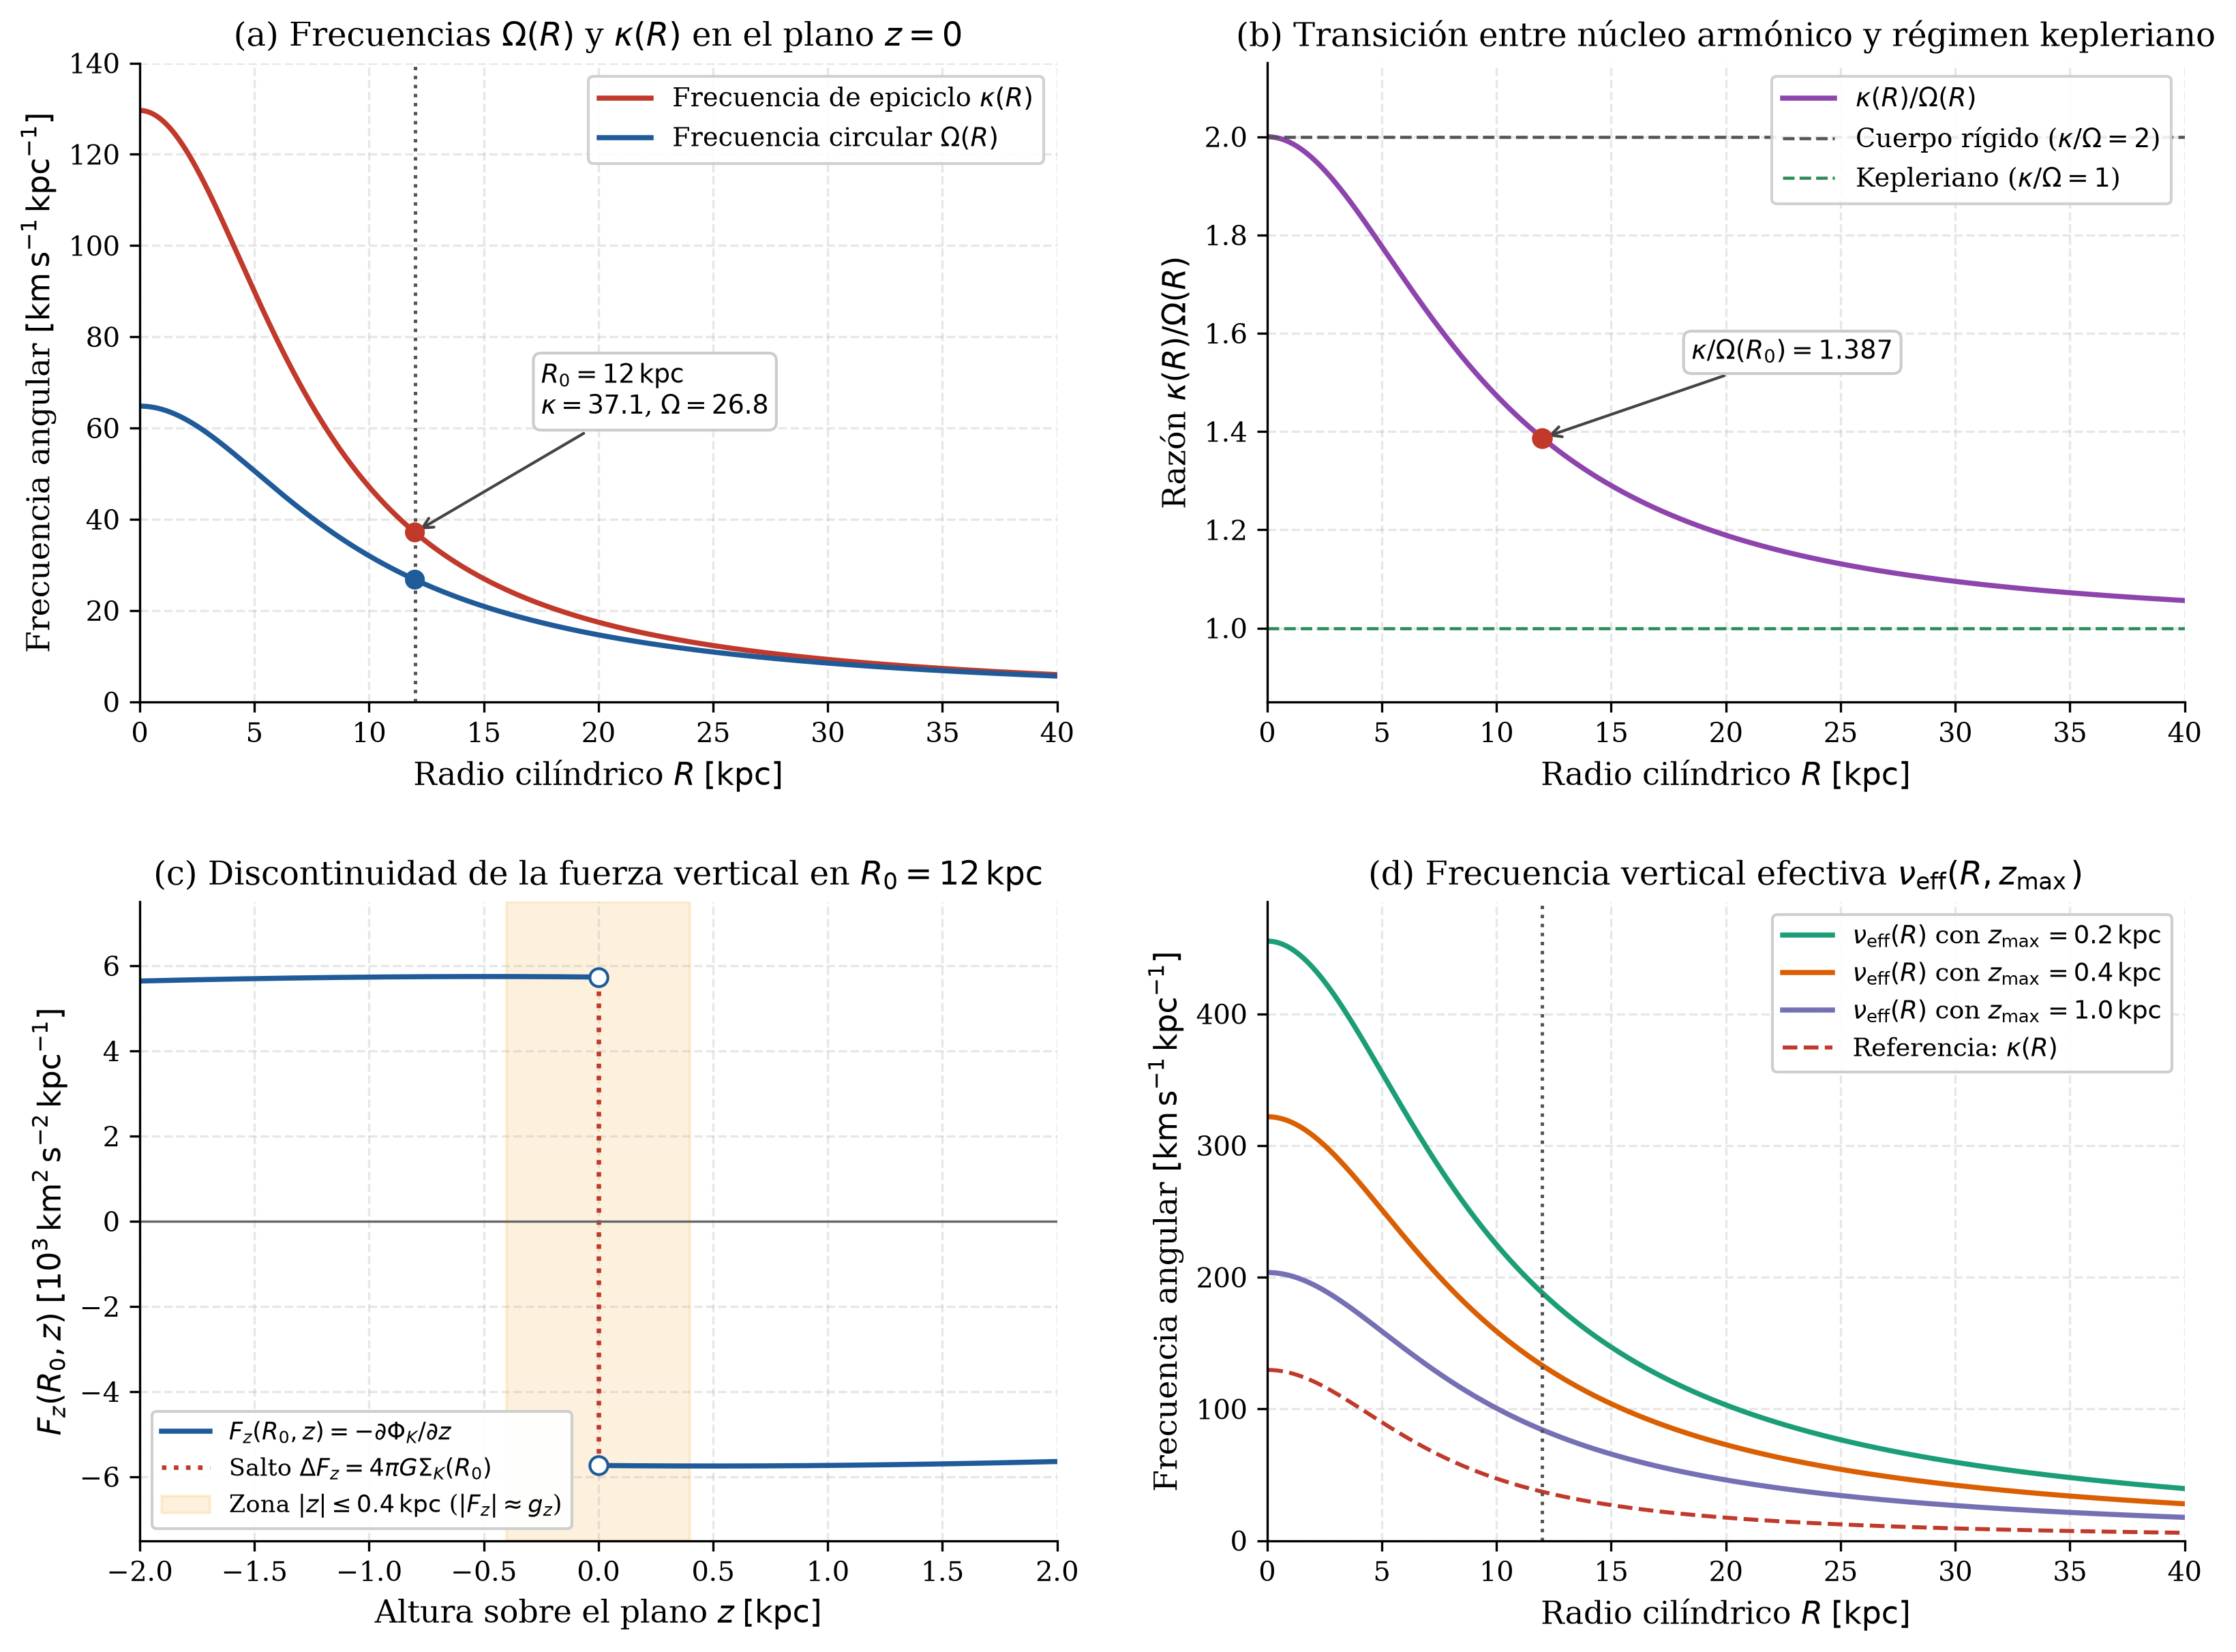
\includegraphics[width=0.98\textwidth]{fig2_kuzmin_frequencies.png}
    \caption{Predicciones analíticas para el disco de Kuzmin. (a) $\kappa(R)$ y $\Omega(R)$ en $z=0$. (b) Razón $\kappa(R)/\Omega(R)$ entre el límite armónico ($2$) y el kepleriano ($1$). (c) Salto de $F_z(R_0, z)$ en $z = 0$ y zona $|z|\le 0.4\,\mathrm{kpc}$ donde $|F_z| \approx g_z$. (d) $\nu_{\mathrm{eff}}(R, z_{\max})$ para tres amplitudes pequeñas junto con $\kappa(R)$.}
    \label{fig:kuzmin_freq}
\end{figure}

La Figura~\ref{fig:kuzmin_freq} resume las predicciones analíticas obtenidas para las frecuencias radial y vertical del disco de Kuzmin. Recordando que en la Sección~1.1 se obtuvo $\kappa(R)/\Omega(R) = \sqrt{1 + 3a_d^2/(R^2 + a_d^2)}$, entonces a partir de las gráficas~(a)--(b) se identifican tres regímenes radiales:
\begin{itemize}
    \item \textbf{Centro ($R \ll a_d$):} $\Sigma_K$ es casi uniforme, $\Omega \approx \sqrt{GM_d/a_d^3}$ es constante (potencial armónico) y $\kappa/\Omega \to 2$ (dos oscilaciones radiales por vuelta).
    \item \textbf{Exterior ($R \gg a_d$):} casi toda la masa queda interior a $R$, el potencial tiende al de una masa puntual ($\Omega \propto R^{-3/2}$) y $\kappa/\Omega \to 1$ (régimen kepleriano).
    \item \textbf{Radios intermedios ($0 < R < \infty$):} siempre $1 < \kappa/\Omega < 2$. En general esta razón no es racional, así que se forma una órbita no cerrada acotada entre un pericentro y un apocentro.
\end{itemize}

Por su parte, la gráfica~(c) ilustra el salto de $F_z(R_0, z)$ en $z = 0$ y la región cercana al plano donde $|F_z| \approx g_z(R_0)$. A partir de la expresión para $\nu_{\mathrm{eff}}(R, z_{\max})$ y de la gráfica~(d) se observan tres comportamientos principales:
\begin{itemize}
    \item \textbf{Dependencia radial:} $\nu_{\mathrm{eff}}$ es máxima en $R = 0$ y decrece hacia afuera como $(R^2 + a_d^2)^{-3/4}$, siguiendo la caída de la densidad superficial local $\Sigma_K(R)$. A menor masa local en el plano, menor es $g_z$ y más lenta la oscilación vertical.
    \item \textbf{Dependencia con $z_{\max}$:} por ser un movimiento anarmónico, $\nu_{\mathrm{eff}} \propto z_{\max}^{-1/2}$: a menor amplitud vertical, mayor frecuencia (divergiendo cuando $z_{\max} \to 0$, coherente con la $\delta(z)$).
    \item \textbf{Jerarquía de frecuencias ($\nu_{\mathrm{eff}} > \kappa > \Omega$):} para alturas pequeñas ($z_{\max} \le 1\,\mathrm{kpc}$), las curvas de $\nu_{\mathrm{eff}}(R)$ quedan siempre por encima de $\kappa(R)$, es decir, $T_z < T_\kappa < T_{\mathrm{orb}}$. Esto implica que la estrella completa varias oscilaciones verticales por cada ciclo radial (en $R_0 = 12\,\mathrm{kpc}$ con $z_{\max} = 0.4\,\mathrm{kpc}$, $\nu_{\mathrm{eff}}/\kappa \approx 3.6$), reflejo de una fuerza restauradora vertical más intensa cerca del plano del disco.
\end{itemize}

% =============================================================================
% Numeral 2: Integración numérica en el disco de Kuzmin
% =============================================================================
\section{Integración numérica de órbitas en el potencial de Kuzmin}

Para integrar $\mathrm{d}^2\mathbf{r}/\mathrm{d}t^2 = -\nabla\Phi_K(\mathbf{r})$ se trabaja en coordenadas cartesianas $(x, y, z)$, lo que evita singularidades en $R = 0$. Sustituyendo $R^2 = x^2 + y^2$ en el potencial de Kuzmin y definiendo $D_K \equiv \sqrt{x^2 + y^2 + (a_d + |z|)^2}$, este se escribe como:
\begin{equation}
    \Phi_K(x, y, z) = -G M_d\left[x^2 + y^2 + (a_d + |z|)^2\right]^{-1/2} = -G M_d\,(D_K^2)^{-1/2}.
\end{equation}
Aplicando la regla de la cadena para cualquier coordenada cartesiana $q_i \in \{x, y, z\}$, cada componente de la aceleración $\mathbf{a} = -\nabla\Phi_K$ cumple:
\begin{equation}
    a_i = -\frac{\partial \Phi_K}{\partial q_i}
    = G M_d\left(-\frac{1}{2}\right)(D_K^2)^{-3/2}\,\frac{\partial (D_K^2)}{\partial q_i}
    = -\frac{G M_d}{2 D_K^3}\,\frac{\partial (D_K^2)}{\partial q_i}.
\end{equation}
Evaluando las derivadas parciales de $D_K^2 = x^2 + y^2 + (a_d + |z|)^2$ respecto a $x$, $y$ y $z$ (usando $\mathrm{d}|z|/\mathrm{d}z = \operatorname{sgn}(z)$ para $z \neq 0$), se obtienen las tres componentes exactas:
\begin{align}
    a_x &= -\frac{G M_d}{2 D_K^3}\,(2x) = -\frac{G M_d\,x}{D_K^3}, \nonumber \\
    a_y &= -\frac{G M_d}{2 D_K^3}\,(2y) = -\frac{G M_d\,y}{D_K^3}, \\
    a_z &= -\frac{G M_d}{2 D_K^3}\cdot 2(a_d + |z|)\,\operatorname{sgn}(z) = -\frac{G M_d\,(a_d + |z|)\,\operatorname{sgn}(z)}{D_K^3}, \nonumber
\end{align}
fijando $\operatorname{sgn}(0) = 0$ para que sobre el plano $z = 0$ la aceleración vertical sea exactamente nula por simetría.

\paragraph{Método numérico.}
\mbox{}\\[0.4em]
Discretizando el tiempo en pasos uniformes $t_n = n\,\Delta t$, se implemento el algoritmo de diferencias finitas centradas de segundo orden Velocity Verlet (Binney \& Tremaine, 2008, \S 3.4.1), que avanza cada paso en tres etapas (medio paso en velocidad, paso completo en posición y medio paso final en velocidad):
\begin{equation}
    \mathbf{v}_{n+1/2} = \mathbf{v}_n + \frac{1}{2}\mathbf{a}(\mathbf{r}_n)\,\Delta t, \qquad
    \mathbf{r}_{n+1} = \mathbf{r}_n + \mathbf{v}_{n+1/2}\,\Delta t, \qquad
    \mathbf{v}_{n+1} = \mathbf{v}_{n+1/2} + \frac{1}{2}\mathbf{a}(\mathbf{r}_{n+1})\,\Delta t.
\end{equation}
Se escoge Velocity Verlet porque es reversible en el tiempo y simpléctico: los errores en la energía $E$ y el momento angular $L_z$ no presentan deriva secular sino que permanecen acotados. Con pasos pequeños ($\Delta t = 5\times 10^{-5}\,t_u$ en equilibrio y $\Delta t = 2.5\times 10^{-5}\,t_u$ en las órbitas perturbadas, más de $1800$ pasos por oscilación vertical), los cruces por $z = 0$ se integran de forma estable.

\subsection{Órbita en configuración de equilibrio}

Se escoge el radio de estudio $R_0 = 12.0\,\mathrm{kpc}$ ($1.5\,a_d$), justo fuera del pico de $v_c$ ($R_{\mathrm{max}} \approx 11.3\,\mathrm{kpc}$), donde la razón $\kappa/\Omega = 1.387$ está en el régimen intermedio entre el núcleo armónico y el límite kepleriano.

Teniendo en cuenta los resultados del punto anterior, $v_c(R) = \sqrt{GM_d R^2/(R^2 + a_d^2)^{3/2}}$ y $\Omega(R) = v_c(R)/R$, para $R_0 = 12.0\,\mathrm{kpc}$ la teoría predice una velocidad circular $v_c(R_0) = 321.28\,\mathrm{km\,s^{-1}}$, frecuencia $\Omega(R_0) = 26.77\,\mathrm{km\,s^{-1}\,kpc^{-1}}$ y periodo orbital $T_{\mathrm{orb}} = 2\pi/\Omega = 0.2347\,t_u \approx 229.5\,\mathrm{Myr}$. Se fijan entonces las condiciones iniciales en equilibrio circular sobre $z = 0$:
\begin{equation}
    \mathbf{r}(0) = (12.0,\; 0,\; 0)\,\mathrm{kpc}, \qquad
    \mathbf{v}(0) = (0,\; 321.2838,\; 0)\,\mathrm{km\,s^{-1}}.
\end{equation}

\begin{figure}[H]
    \centering
    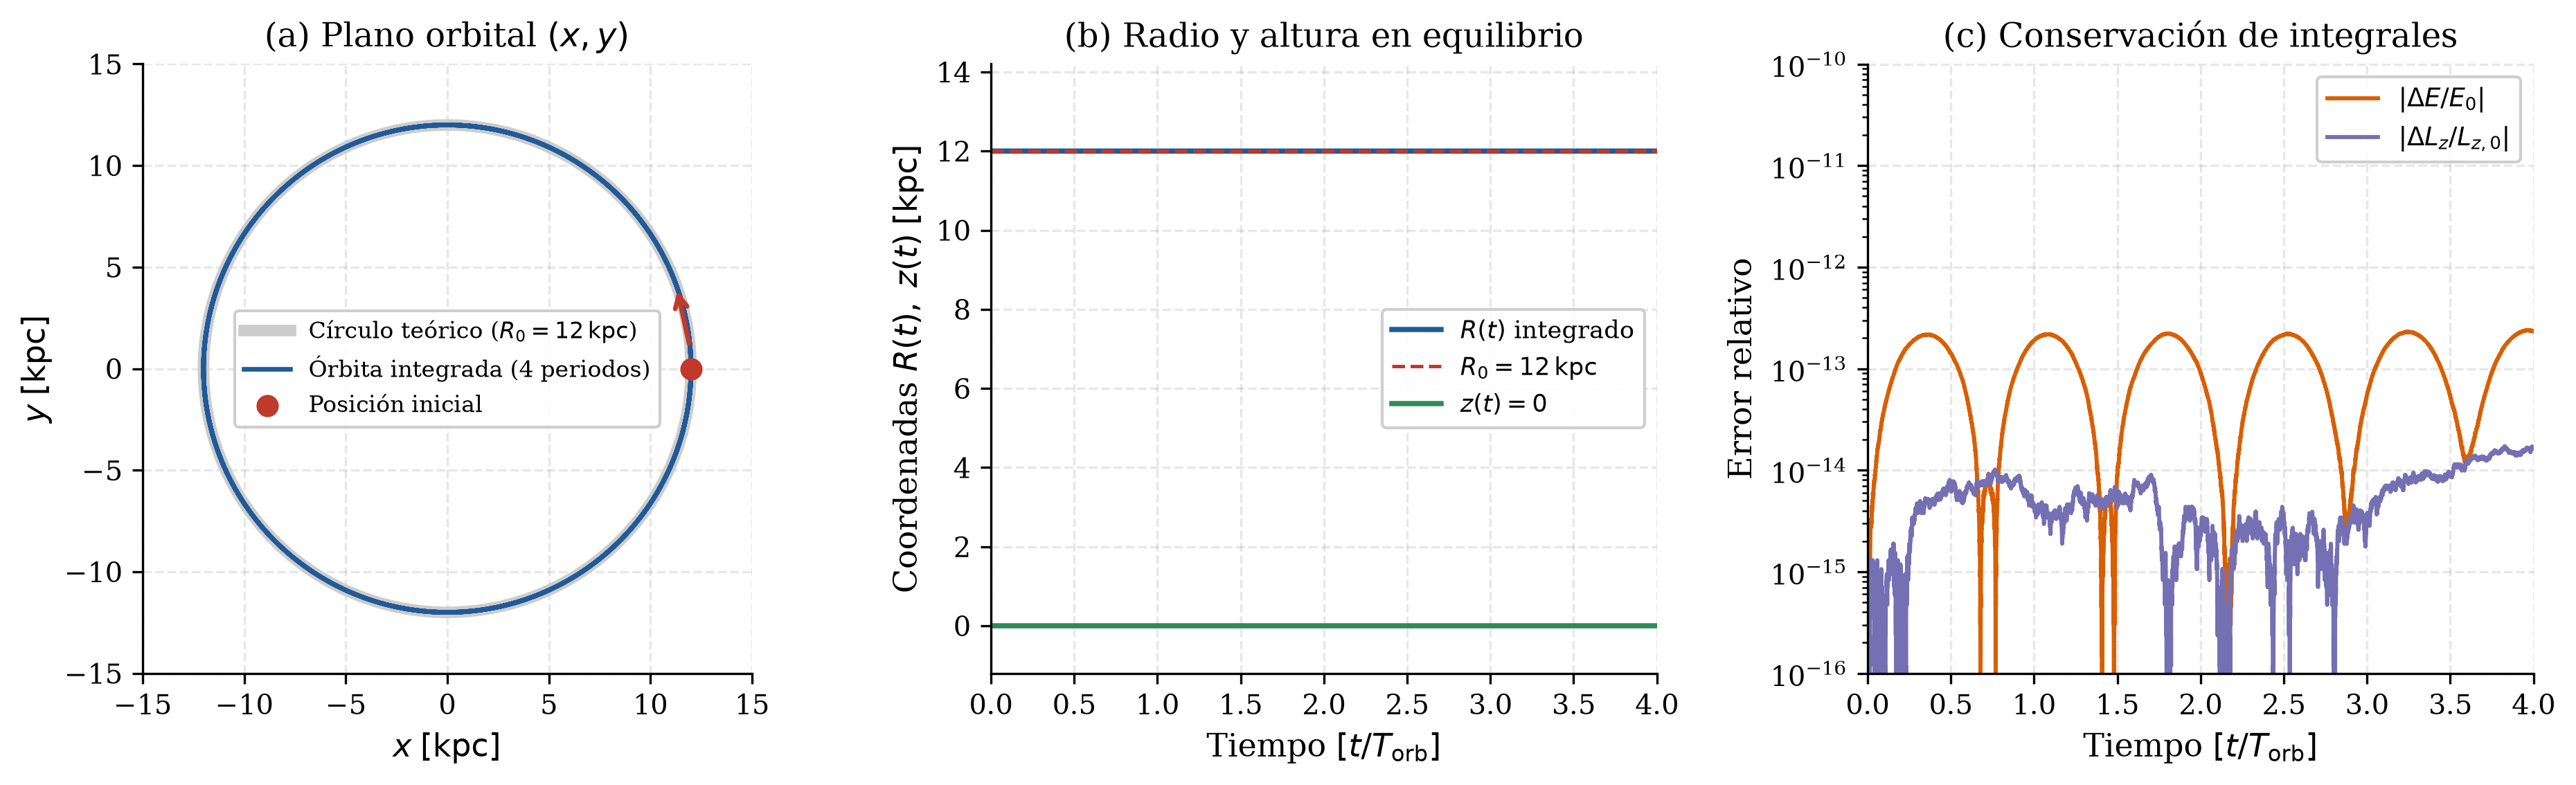
\includegraphics[width=0.99\textwidth]{fig3_equilibrium_orbit.png}
    \caption{Órbita de equilibrio en $R_0 = 12\,\mathrm{kpc}$ integrada durante $4$ periodos orbitales ($\approx 918\,\mathrm{Myr}$). (a) Plano $(x,y)$ frente al círculo teórico. (b) Evolución de $R(t)$ y $z(t)$. (c) Errores relativos en $E$ y $L_z$.}
    \label{fig:eq_orbit}
\end{figure}

La Figura~\ref{fig:eq_orbit} muestra los resultados tras $4$ periodos orbitales ($\approx 0.939\,t_u$). Tal como predice el modelo, la trayectoria es circular y confinada al plano $z = 0$: $\max|R(t) - R_0| = 5.6\times 10^{-6}\,\mathrm{kpc}$, $z(t) = 0$ en todo instante y el periodo medido coincide con el teórico ($T_{\mathrm{orb,num}} = 0.234678\,t_u$). Los errores relativos se mantienen acotados en $|\Delta E/E_0| \le 2.4\times 10^{-13}$ y $|\Delta L_z/L_{z,0}| \le 1.7\times 10^{-14}$ (gráfica~c).

\subsection{Órbita con pequeñas perturbaciones radial y vertical}

Para generar oscilaciones pequeñas alrededor del equilibrio sin salir del régimen lineal, se modifica el estado inicial así:
\begin{itemize}
    \item \textbf{Perturbación radial en velocidad:} se introduce $\delta v_R = 0.05\,v_c(R_0) \approx 16.06\,\mathrm{km\,s^{-1}}$ manteniendo $R(0) = R_0$ y $v_\phi(0) = v_c(R_0)$. Elegir una perturbación del $5\%$ en $v_R$ garantiza una amplitud pequeña y deja intacto el momento angular $L_z = R_0 v_c(R_0)$, así que el radio guía teórico sigue siendo $R_g = R_0$. Al resolver el oscilador armónico radial $\ddot{x} = -\kappa^2 x$ con $x(0) = 0$ y $\dot{x}(0) = \delta v_R$, la teoría predice:
    \begin{equation}
        R(t) \approx R_0 + A_R\sin(\kappa t),
        \qquad
        A_R = \frac{\delta v_R}{\kappa(R_0)} \approx 0.433\,\mathrm{kpc}\;\;(3.6\%\text{ de } R_0).
    \end{equation}
    \item \textbf{Perturbación vertical en posición:} se coloca la estrella en $z_0 = 0.40\,\mathrm{kpc}$ con $v_z(0) = 0$. Esta altura es solo $3.3\%$ de $R_0$ ($5\%$ de $a_d$, del mismo orden que la escala vertical del disco delgado $z_0 = 0.3\,\mathrm{kpc}$), así que permanece en la zona donde $|F_z| \approx g_z(R_0)$ (Figura~\ref{fig:kuzmin_freq}c). Además, partir con $v_z(0) = 0$ fija la amplitud máxima $z_{\max} \approx z_0 = 0.40\,\mathrm{kpc}$, lo que permite evaluar directamente $\nu_{\mathrm{eff}}(R_0, z_{\max}) = \frac{\pi}{2}\sqrt{g_z(R_0)/(2z_{\max})}$ y facilita luego la comparación con el halo.
\end{itemize}

Con ambas perturbaciones, las condiciones iniciales quedan fijadas en:
\begin{equation}
    \mathbf{r}(0) = (12.0,\; 0,\; 0.40)\,\mathrm{kpc}, \qquad
    \mathbf{v}(0) = (16.0642,\; 321.2838,\; 0)\,\mathrm{km\,s^{-1}}.
\end{equation}
Se integra esta órbita durante $5$ periodos orbitales ($\approx 1.173\,t_u \approx 1.15\,\mathrm{Gyr}$). Las integrales se conservan bien pese a los múltiples cruces por $z = 0$: $|\Delta L_z/L_{z,0}| \le 2.9\times 10^{-14}$ y $|\Delta E/E_0| \le 2.7\times 10^{-4}$, sin deriva secular.

\begin{figure}[H]
    \centering
    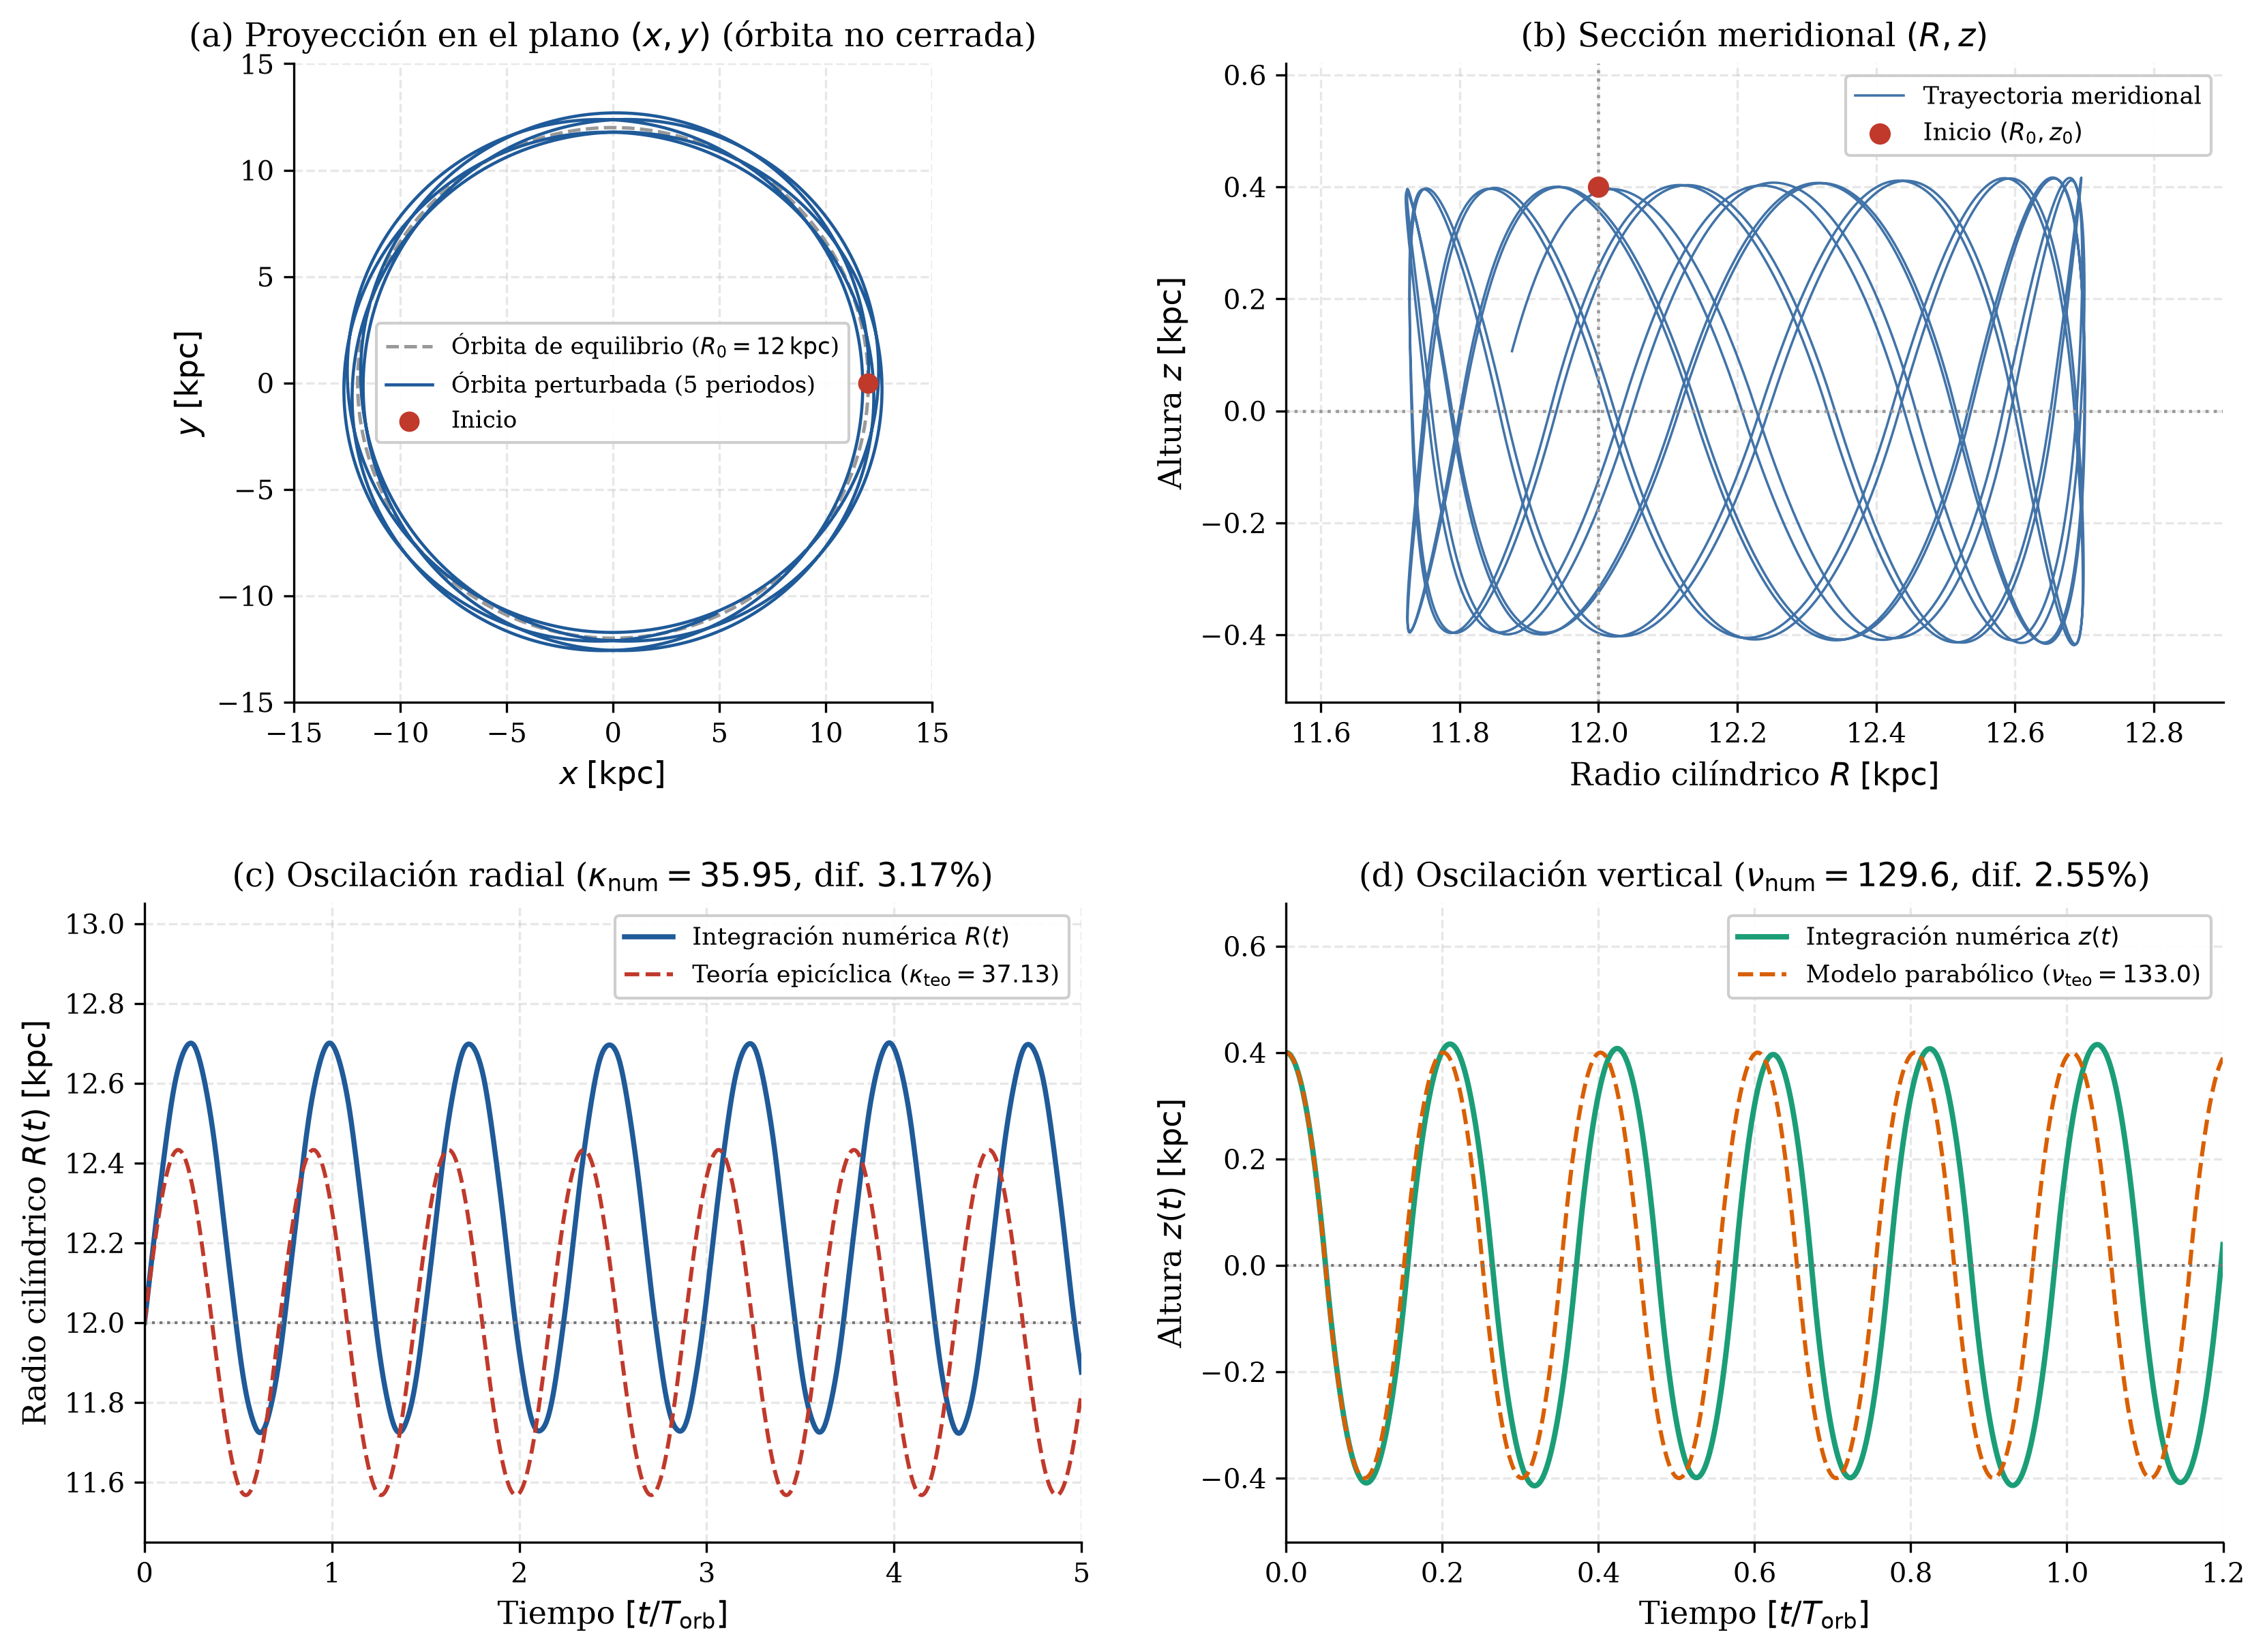
\includegraphics[width=0.98\textwidth]{fig4_perturbed_orbit.png}
    \caption{Órbita perturbada en el disco de Kuzmin durante $5$ periodos orbitales ($\delta v_R = 0.05\,v_c$, $z_0 = 0.40\,\mathrm{kpc}$). (a) Órbita no cerrada en el plano $(x,y)$. (b) Sección meridional $(R,z)$. (c) $R(t)$ numérico frente a la predicción epicíclica. (d) $z(t)$ numérico frente al modelo parabólico a trozos en los primeros $1.2$ periodos orbitales.}
    \label{fig:pert_orbit}
\end{figure}

\begin{table}[H]
    \centering
    \caption{Comparación entre las predicciones analíticas en $(R_0 = 12\,\mathrm{kpc}, z = 0)$ y los valores medidos en la simulación perturbada del disco de Kuzmin.}
    \label{tab:part2}
    \small
    \setlength{\tabcolsep}{7pt}
    \begin{tabular}{@{}lccc@{}}
        \toprule
        Magnitud & Predicción analítica & Simulación numérica & Dif.\ relativa \\
        \midrule
        Frecuencia de epiciclo $\kappa\;[\mathrm{km\,s^{-1}\,kpc^{-1}}]$ & $37.13$ & $35.95$ & $3.17\%$ \\
        Periodo radial $T_\kappa\;[\mathrm{Myr}]$ & $165.5$ & $170.9$ & $3.26\%$ \\
        Amplitud radial $A_R\;[\mathrm{kpc}]$ & $0.433$ & $0.489$ & --- \\
        Frecuencia vertical efectiva $\nu_{\mathrm{eff}}\;[\mathrm{km\,s^{-1}\,kpc^{-1}}]$ & $133.0$ & $129.6$ & $2.55\%$ \\
        Periodo vertical $T_z\;[\mathrm{Myr}]$ & $46.20$ & $47.40$ & $2.61\%$ \\
        \bottomrule
    \end{tabular}
\end{table}

La Figura~\ref{fig:pert_orbit} y la Tabla~\ref{tab:part2} comparan la integración numérica con la teoría:
\begin{itemize}
    \item \textbf{Geometría de la órbita:} en $(x,y)$ se forma una órbita no cerrada (gráfica~a): en $5$ vueltas azimutales hay casi $7$ ciclos radiales, acorde con $\kappa/\Omega \approx 1.39$. En el plano meridional $(R,z)$ (gráfica~b), la órbita permanece acotada en una región regular alrededor de $(R_0, 0)$.
    \item \textbf{Frecuencias radial y vertical:} la frecuencia radial medida en los picos de $R(t)$ (gráfica~c) es $\kappa_{\mathrm{num}} = 35.95\,\mathrm{km\,s^{-1}\,kpc^{-1}}$, a $3.17\%$ del valor analítico $\kappa_{\mathrm{teo}} = 37.13$. La frecuencia vertical medida por cruces ascendentes de $z = 0$ es $\nu_{\mathrm{num}} = 129.6\,\mathrm{km\,s^{-1}\,kpc^{-1}}$, a $2.55\%$ de la predicción parabólica obtenida en la Sección~1.2 ($\nu_{\mathrm{teo}} = 133.0$). En la gráfica~(d) se distinguen además los arcos parabólicos y el cambio de curvatura al cruzar $z = 0$.
    \item \textbf{Efectos no lineales y acoplamiento entre $R$ y $z$:} en la gráfica~(c) la curva numérica aparece desplazada por encima de la predicción epicíclica ($R_{\text{medio}} \approx 12.24\,\mathrm{kpc}$, entre $11.73$ y $12.70\,\mathrm{kpc}$, frente a una oscilación simétrica alrededor de $12.0\,\mathrm{kpc}$). Aquí se manifiestan dos factores reales que la teoría lineal desprecia: por un lado, el acoplamiento vertical-radial, pues al oscilar con $|z| \le 0.4\,\mathrm{kpc}$ aumenta el denominador $[R^2 + (a_d + |z|)^2]^{3/2}$ y se debilita la atracción radial con el mismo $L_z$, desplazando el equilibrio efectivo hacia afuera; por otro, la asimetría del pozo efectivo $\Phi_{\mathrm{eff}}(R,0)$, cuya barrera centrífuga interior ($\propto L_z^2/2R^2$) es más empinada que la pared exterior, lo que favorece excursiones mayores hacia radios grandes.
    \item \textbf{Acumulación de desfase:} como $\kappa(R)$ y $|F_z(R,z)|$ decrecen al desplazarse el radio medio hacia afuera y salir de $z = 0$, tanto $\kappa_{\mathrm{num}}$ como $\nu_{\mathrm{num}}$ resultan $\sim 2.5\%$--$3\%$ menores que los valores teóricos evaluados exactamente en $(R_0, 0)$. Aunque esta discrepancia es pequeña en un solo ciclo, se acumula con el tiempo y explica el desfase progresivo visible entre las curvas numéricas y analíticas en las gráficas~(c) y~(d), mostrando cómo los términos despreciados por el modelo idealizado emergen en la dinámica completa.
\end{itemize}

% =============================================================================
% Numeral 3: Disco + Halo oblato de Miyamoto-Nagai
% =============================================================================
\section{Inclusión del halo de materia oscura}

Ahora se agrega un halo de materia oscura modelado con el potencial de Miyamoto-Nagai (Binney \& Tremaine, 2008, \S 2.3.1, Ec.~2.69a, p.~73):
\begin{equation}
    \Phi_h(R, z) = -\frac{G M_h}{\sqrt{R^2 + \left(a_h + \sqrt{z^2 + b_h^2}\right)^2}}.
    \label{eq:phi_mn}
\end{equation}
Para obtener su densidad volumétrica asociada $\rho_h(R, z)$ se aplica la ecuación de Poisson en coordenadas cilíndricas con simetría axial ($\partial/\partial\phi = 0$; Binney \& Tremaine, 2008, \S 2.1, Ec.~2.10, p.~57):
\begin{equation}
    \nabla^2\Phi_h = \frac{1}{R}\frac{\partial}{\partial R}\!\left(R\frac{\partial \Phi_h}{\partial R}\right) + \frac{\partial^2 \Phi_h}{\partial z^2} = 4\pi G \rho_h(R, z).
\end{equation}
Definiendo $B \equiv \sqrt{z^2 + b_h^2}$, $A \equiv a_h + B$ y $D_h \equiv \sqrt{R^2 + A^2}$, de modo que $\Phi_h = -G M_h\,D_h^{-1}$, $B^2 - z^2 = b_h^2$ y $\mathrm{d}A/\mathrm{d}z = \mathrm{d}B/\mathrm{d}z = z/B$.

Primero, calculando el término radial del laplaciano mediante la regla de la cadena y la regla del cociente:
\begin{gather}
    \frac{\partial \Phi_h}{\partial R} = \frac{G M_h R}{D_h^3}, \nonumber \\[3pt]
    \frac{1}{R}\frac{\partial}{\partial R}\!\left(\frac{G M_h R^2}{D_h^3}\right)
    = \frac{G M_h}{R}\,\frac{2R\,D_h^3 - 3R^3 D_h}{D_h^6}
    = G M_h\,\frac{2D_h^2 - 3R^2}{D_h^5}
    = G M_h\,\frac{2A^2 - R^2}{D_h^5}.
\end{gather}
En dirección vertical, derivando respecto a $z$ y usando $A/B = 1 + a_h/B$:
\begin{equation}
    \frac{\partial \Phi_h}{\partial z}
    = G M_h\,\frac{A}{D_h^3}\,\frac{z}{B}
    = G M_h\left(z + \frac{a_h z}{B}\right)D_h^{-3}.
\end{equation}
Derivando una segunda vez respecto a $z$ (usando $\frac{\mathrm{d}}{\mathrm{d}z}(z/B) = (B - z^2/B)/B^2 = b_h^2/B^3$ y $\partial(D_h^{-3})/\partial z = -3 A z/(B D_h^5)$):
\begin{align}
    \frac{\partial^2 \Phi_h}{\partial z^2}
    &= G M_h\left[\left(1 + \frac{a_h b_h^2}{B^3}\right)\frac{1}{D_h^3}
    - \frac{3 A^2 z^2}{B^2 D_h^5}\right] \nonumber \\
    &= \frac{G M_h}{B^3 D_h^5}\left[(B^3 + a_h b_h^2)D_h^2 - 3 A^2 B z^2\right].
\end{align}
Sumando las contribuciones radial y vertical, sustituyendo $D_h^2 = R^2 + A^2$ y usando $B^2 - z^2 = b_h^2$:
\begin{align}
    \nabla^2\Phi_h
    &= \frac{G M_h}{B^3 D_h^5}\left[B^3(2A^2 - R^2) + (B^3 + a_h b_h^2)(R^2 + A^2) - 3 A^2 B z^2\right] \nonumber \\
    &= \frac{G M_h}{B^3 D_h^5}\left[a_h b_h^2 R^2 + 3 A^2 B(B^2 - z^2) + a_h b_h^2 A^2\right] \nonumber \\
    &= \frac{G M_h b_h^2}{B^3 D_h^5}\left[a_h R^2 + (a_h + 3B)A^2\right].
\end{align}
Igualando a la ecuación de Poisson, $4\pi G\rho_h = \nabla^2\Phi_h$, despejando $\rho_h$ (donde se cancela $G$) y sustituyendo de vuelta $B = \sqrt{z^2 + b_h^2}$, $A = a_h + B$ y $D_h = \sqrt{R^2 + A^2}$, se obtiene la densidad volumétrica de Miyamoto-Nagai:
\begin{gather}
    4\pi G\rho_h = \frac{G M_h b_h^2}{B^3 D_h^5}\left[a_h R^2 + (a_h + 3B)A^2\right]
    \quad \Longrightarrow \quad
    \rho_h(R, z) = \frac{b_h^2 M_h}{4\pi}\,\frac{a_h R^2 + (a_h + 3B)A^2}{D_h^5 B^3}, \nonumber \\[6pt]
    \boxed{\rho_h(R, z) = \frac{b_h^2 M_h}{4\pi}\,
    \frac{a_h R^2 + \left(a_h + 3\sqrt{z^2 + b_h^2}\right)\left(a_h + \sqrt{z^2 + b_h^2}\right)^2}
         {\left[R^2 + \left(a_h + \sqrt{z^2 + b_h^2}\right)^2\right]^{5/2} (z^2 + b_h^2)^{3/2}}}.
    \label{eq:rho_mn}
\end{gather}

\subsection{Eje de achatamiento y elección de los parámetros del halo}

Como $\Phi_h$ y $\rho_h$ dependen solo de $R$ y $z$, entonces el sistema tiene simetría axial respecto al \textbf{eje $z$}. cuando $a_h = 0$ se recupera el potencial esférico de Plummer y cuando $b_h = 0$ el disco plano de Kuzmin; para cualquier $a_h > 0$ y $b_h > 0$, la distribución es más extensa en el plano ecuatorial que en dirección polar, es decir, un esferoide achatado a lo largo del eje $z$ (eje perpendicular al plano del disco).

La razón $b_h / a_h$ determina el grado de achatamiento (Binney \& Tremaine, 2008, Fig.~2.7, p.~74): $b_h/a_h \sim 0.2$ corresponde a un disco delgado y $b_h/a_h > 1$ a distribuciones más redondeadas, apropiadas para un halo. Así que se eligen:
\begin{equation}
    M_h = 2.5 \times 10^{12}\,M_\odot = 250\,M_u, \qquad
    a_h = 8.0\,\mathrm{kpc}, \qquad
    b_h = 20.0\,\mathrm{kpc}.
\end{equation}
Esta elección se justifica en tres criterios:
\begin{itemize}
    \item \textbf{Masa ($M_h = 5\,M_d$):} en los modelos galácticos presentados en Binney \& Tremaine (2008, Tabla~2.3, p.~113), el halo domina la masa total sobre el disco por aproximadamente un orden de magnitud; se elige $M_h/M_d = 5$ para que el halo sea claramente dominante sin llevar las velocidades de rotación a valores extremos.
    \item \textbf{Extensión ($a_h + b_h = 28\,\mathrm{kpc} > a_d = 8\,\mathrm{kpc}$):} al tener una escala radial mucho mayor que el disco, el halo sostiene la curva de rotación en los radios externos y evita la caída kepleriana temprana.
    \item \textbf{Achatamiento ($b_h/a_h = 2.5$):} produce contornos de isodensidad oblatos en $z$ con razón de ejes $q_\rho = z_m / R_m \approx 0.75$ entre $R = 12$ y $30\,\mathrm{kpc}$.
\end{itemize}

\begin{figure}[H]
    \centering
    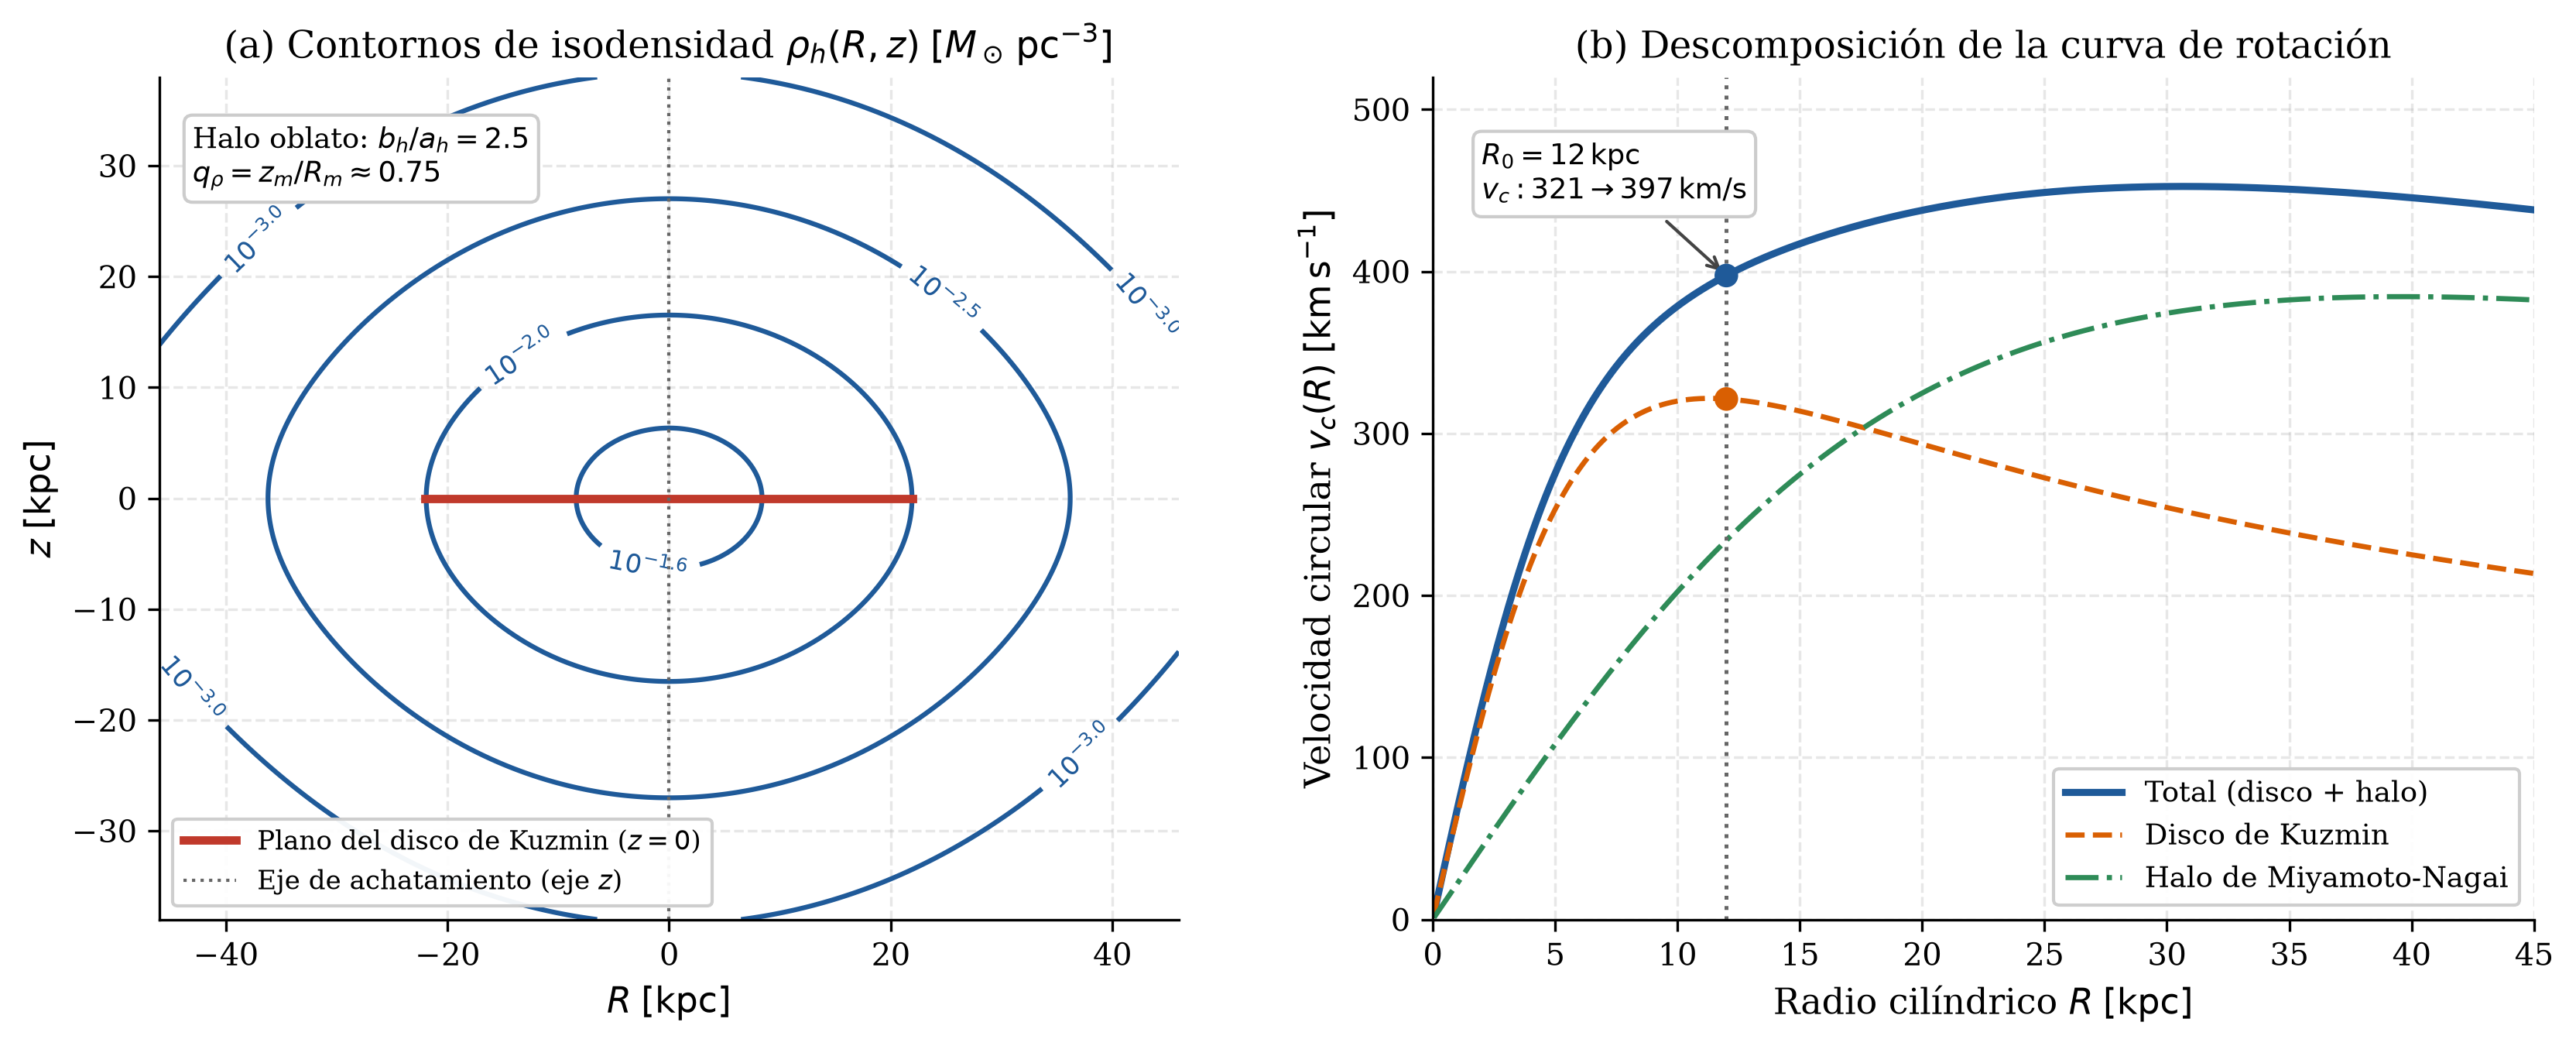
\includegraphics[width=0.98\textwidth]{fig5_halo_structure_and_vc.png}
    \caption{Halo oblato de Miyamoto-Nagai ($M_h = 2.5\times 10^{12}\,M_\odot$, $a_h = 8\,\mathrm{kpc}$, $b_h = 20\,\mathrm{kpc}$). (a) Contornos de isodensidad $\rho_h(R, z)$ mostrando el achatamiento en el eje $z$ ($q_\rho \approx 0.75$). (b) Descomposición de la curva de rotación total $v_{c,\mathrm{tot}} = \sqrt{v_{c,d}^2 + v_{c,h}^2}$.}
    \label{fig:halo_vc}
\end{figure}

La gráfica~(a) confirma el achatamiento oblato de los contornos de isodensidad $\rho_h(R, z)$ a lo largo del eje $z$ ($q_\rho \approx 0.75$), mientras que la gráfica~(b) muestra cómo el aporte del halo mantiene elevada la curva de rotación total $v_{c,\mathrm{tot}} = \sqrt{v_{c,d}^2 + v_{c,h}^2}$ más allá de $R_0 = 12\,\mathrm{kpc}$, compensando el decaimiento del disco.

\subsection{Predicción teórica del cambio en las frecuencias \texorpdfstring{$\kappa$ y $\nu$}{kappa y nu}}

El potencial combinado es $\Phi_{\mathrm{tot}}(R,z) = \Phi_K(R,z) + \Phi_h(R,z)$. Como $v_c^2$, $\Omega^2$ y $\kappa^2$ dependen linealmente de las derivadas radiales de $\Phi$, las contribuciones al cuadrado de cada componente se suman directamente ($v_{c,\mathrm{tot}}^2 = v_{c,d}^2 + v_{c,h}^2$, $\Omega_{\mathrm{tot}}^2 = \Omega_d^2 + \Omega_h^2$ y $\kappa_{\mathrm{tot}}^2 = \kappa_d^2 + \kappa_h^2$).

En el plano $z = 0$, el potencial tridimensional del halo adopta exactamente la misma dependencia radial que el disco de Kuzmin, con escala efectiva $s_h \equiv a_h + b_h$:
\begin{equation}
    \Phi_h(R, 0) = -\frac{G M_h}{\sqrt{R^2 + (a_h + b_h)^2}} = -\frac{G M_h}{\sqrt{R^2 + s_h^2}}.
\end{equation}
Como $\Omega_h^2(R) = \frac{1}{R}(\partial\Phi_h/\partial R)_{z=0}$ y $\kappa_h^2(R) = (\partial^2\Phi_h/\partial R^2)_{z=0} + \frac{3}{R}(\partial\Phi_h/\partial R)_{z=0}$ solo involucran derivadas radiales evaluadas en $z = 0$, sus expresiones salen exactamente reemplazando $(M_d, a_d) \to (M_h, s_h)$ en las expresiones que habiamos obtenido para el potencial de Kuzmin del disco.

En dirección vertical, en cambio, sí interviene la estructura tridimensional del halo. Definiendo $B \equiv \sqrt{z^2 + b_h^2}$ (de modo que $\mathrm{d}B/\mathrm{d}z = z/B$), el potencial se escribe $\Phi_h(R, z) = -GM_h\left[R^2 + (a_h + B)^2\right]^{-1/2}$, y aplicando la regla de la cadena respecto a $z$ se obtiene:
\begin{align}
    \frac{\partial \Phi_h}{\partial z}
    &= -G M_h\left(-\frac{1}{2}\right)\left[R^2 + (a_h + B)^2\right]^{-3/2} \cdot 2(a_h + B)\,\frac{z}{B} \nonumber \\
    &= \underbrace{\frac{GM_h\,(a_h + B)}{B\left[R^2 + (a_h + B)^2\right]^{3/2}}}_{\equiv\, f(R,\,z)}\,z
    = f(R, z)\,z,
\end{align}
que se anula suavemente en $z = 0$ (sin discontinuidad, a diferencia del disco de Kuzmin). Derivando una segunda vez respecto a $z$ mediante la regla del producto:
\begin{equation}
    \frac{\partial^2 \Phi_h}{\partial z^2}
    = \frac{\partial}{\partial z}\!\left[f(R, z)\,z\right]
    = f(R, z)\,\frac{\partial z}{\partial z} + z\,\frac{\partial f(R, z)}{\partial z}
    = f(R, z) + z\,\frac{\partial f(R, z)}{\partial z}.
\end{equation}
Al evaluar esta expresión en $z = 0$, el segundo término se anula por el factor $z = 0$, mientras que $B(0) = \sqrt{0 + b_h^2} = b_h$ y $a_h + b_h = s_h$. Entonces:
\begin{equation}
    \nu_h^2(R) = \left.\frac{\partial^2 \Phi_h}{\partial z^2}\right|_{z=0}
    = f(R, 0) + \underbrace{0\cdot\left.\frac{\partial f}{\partial z}\right|_{z=0}}_{=\,0}
    = \frac{GM_h\,(a_h + b_h)}{b_h\left[R^2 + (a_h + b_h)^2\right]^{3/2}}
    = \frac{GM_h(a_h + b_h)}{b_h(R^2 + s_h^2)^{3/2}}.
\end{equation}
Reuniendo entonces los resultados (con $(M_d, a_d) \to (M_h, s_h)$) y vertical, las tres frecuencias características del halo son:
\begin{gather}
    \boxed{\Omega_h^2(R) = \frac{GM_h}{(R^2 + s_h^2)^{3/2}}}, \qquad
    \boxed{\kappa_h^2(R) = \frac{GM_h(R^2 + 4s_h^2)}{(R^2 + s_h^2)^{5/2}}}, \nonumber \\[4pt]
    \boxed{\nu_h^2(R) = \frac{GM_h(a_h + b_h)}{b_h(R^2 + s_h^2)^{3/2}}}.
    \label{eq:halo_freqs}
\end{gather}

\paragraph{Efecto sobre la frecuencia radial $\kappa$.}
\mbox{}\\[0.4em]
Como $\kappa_{\mathrm{tot}}^2(R) = \kappa_d^2(R) + \kappa_h^2(R)$ y $\kappa_h^2(R) > 0$ para todo $R$, entonces \textbf{$\kappa$ aumenta en todos los radios}. Físicamente, añadir la masa del halo profundiza el pozo radial efectivo y refuerza la fuerza restauradora frente a desplazamientos $\delta R$. Además, como $s_h = 28\,\mathrm{kpc} > a_d = 8\,\mathrm{kpc}$, la fracción de masa aportada por el halo crece con $R$, por tanto el aumento relativo de $\kappa$ es cada vez más pronunciado en radios externos.

\paragraph{Efecto sobre la frecuencia vertical $\nu_{\mathrm{eff}}$.}
\mbox{}\\[0.4em]
Recordando que en la Sección~1.2, para alturas pequeñas ($|z| \ll a_d$), la fuerza vertical por unidad de masa del disco de Kuzmin resultó $F_{z,d}(R, z) \approx -g_{z,d}(R)\,\operatorname{sgn}(z)$ con $g_{z,d}(R) = GM_d a_d/(R^2 + a_d^2)^{3/2} = 2\pi G\Sigma_K(R)$, mientras que el potencial del halo es suave en $z = 0$ y para $|z| \ll b_h$ aporta una fuerza restauradora lineal $F_{z,h}(R, z) \approx -\nu_h^2(R)\,z$ en la misma dirección, al sumar las fuerzas verticales de ambas componentes ($\ddot{z} = -\partial\Phi_{\mathrm{tot}}/\partial z$) se obtiene:
\begin{equation}
    \ddot{z} = F_{z,d}(R, z) + F_{z,h}(R, z)
    \approx -g_{z,d}(R)\,\operatorname{sgn}(z) - \nu_h^2(R)\,z.
    \label{eq:z_ode_tot}
\end{equation}
Al ser mayor la fuerza restauradora en todo $z \neq 0$, entonces la frecuencia vertical también aumenta.

Para el tramo con $z > 0$, la ecuación diferencial queda:
\begin{equation}
    \ddot{z} + \nu_h^2 z = -g_{z,d},
\end{equation}
cuya solución general (homogénea armónica más constante) es:
\begin{equation}
    z(t) = A\cos(\nu_h t) + C\sin(\nu_h t) - \frac{g_{z,d}}{\nu_h^2}.
\end{equation}
Derivando respecto al tiempo, $\dot{z}(t) = -A\nu_h\sin(\nu_h t) + C\nu_h\cos(\nu_h t)$. Al imponer las condiciones iniciales desde la altura máxima, $\dot{z}(0) = 0$ y $z(0) = z_{\max}$:
\begin{align}
    \dot{z}(0) &= -A\nu_h\sin(0) + C\nu_h\cos(0) = \nu_h C = 0
    \quad \Longrightarrow \quad C = 0, \nonumber \\
    z(0) &= A\cos(0) + C\sin(0) - \frac{g_{z,d}}{\nu_h^2} = A - \frac{g_{z,d}}{\nu_h^2} = z_{\max}
    \quad \Longrightarrow \quad A = z_{\max} + \frac{g_{z,d}}{\nu_h^2},
\end{align}
con lo que la trayectoria en el primer tramo resulta:
\begin{equation}
    z(t) = \left(z_{\max} + \frac{g_{z,d}}{\nu_h^2}\right)\cos(\nu_h t) - \frac{g_{z,d}}{\nu_h^2}.
\end{equation}
Al imponer el cruce por el plano medio, $z(t_0) = 0$, se despeja el tiempo de caída $t_0$:
\begin{equation}
    \left(z_{\max} + \frac{g_{z,d}}{\nu_h^2}\right)\cos(\nu_h t_0) = \frac{g_{z,d}}{\nu_h^2}
    \qquad \Longrightarrow \qquad
    t_0 = \frac{1}{\nu_h(R)}\arccos\!\left(\frac{1}{1 + \frac{\nu_h^2(R)\,z_{\max}}{g_{z,d}(R)}}\right).
\end{equation}
Por la misma simetría en cuatro tramos idénticos que en la Sección~1.2, el periodo completo es $T_{z,\mathrm{tot}} = 4\,t_0$ y la frecuencia vertical efectiva resulta:
\begin{equation}
    \boxed{T_{z,\mathrm{tot}}(R, z_{\max}) = \frac{4}{\nu_h(R)}\arccos\!\left(\frac{1}{1 + \frac{\nu_h^2(R)\,z_{\max}}{g_{z,d}(R)}}\right)}, \quad
    \boxed{\nu_{\mathrm{eff,tot}} = \frac{2\pi}{T_{z,\mathrm{tot}}}},
    \label{eq:Tz_tot}
\end{equation}
que en el límite $\nu_h \to 0$ recupera el periodo parabólico del disco aislado, $T_z = 4\sqrt{2z_{\max}/g_{z,d}}$.

\begin{figure}[H]
    \centering
    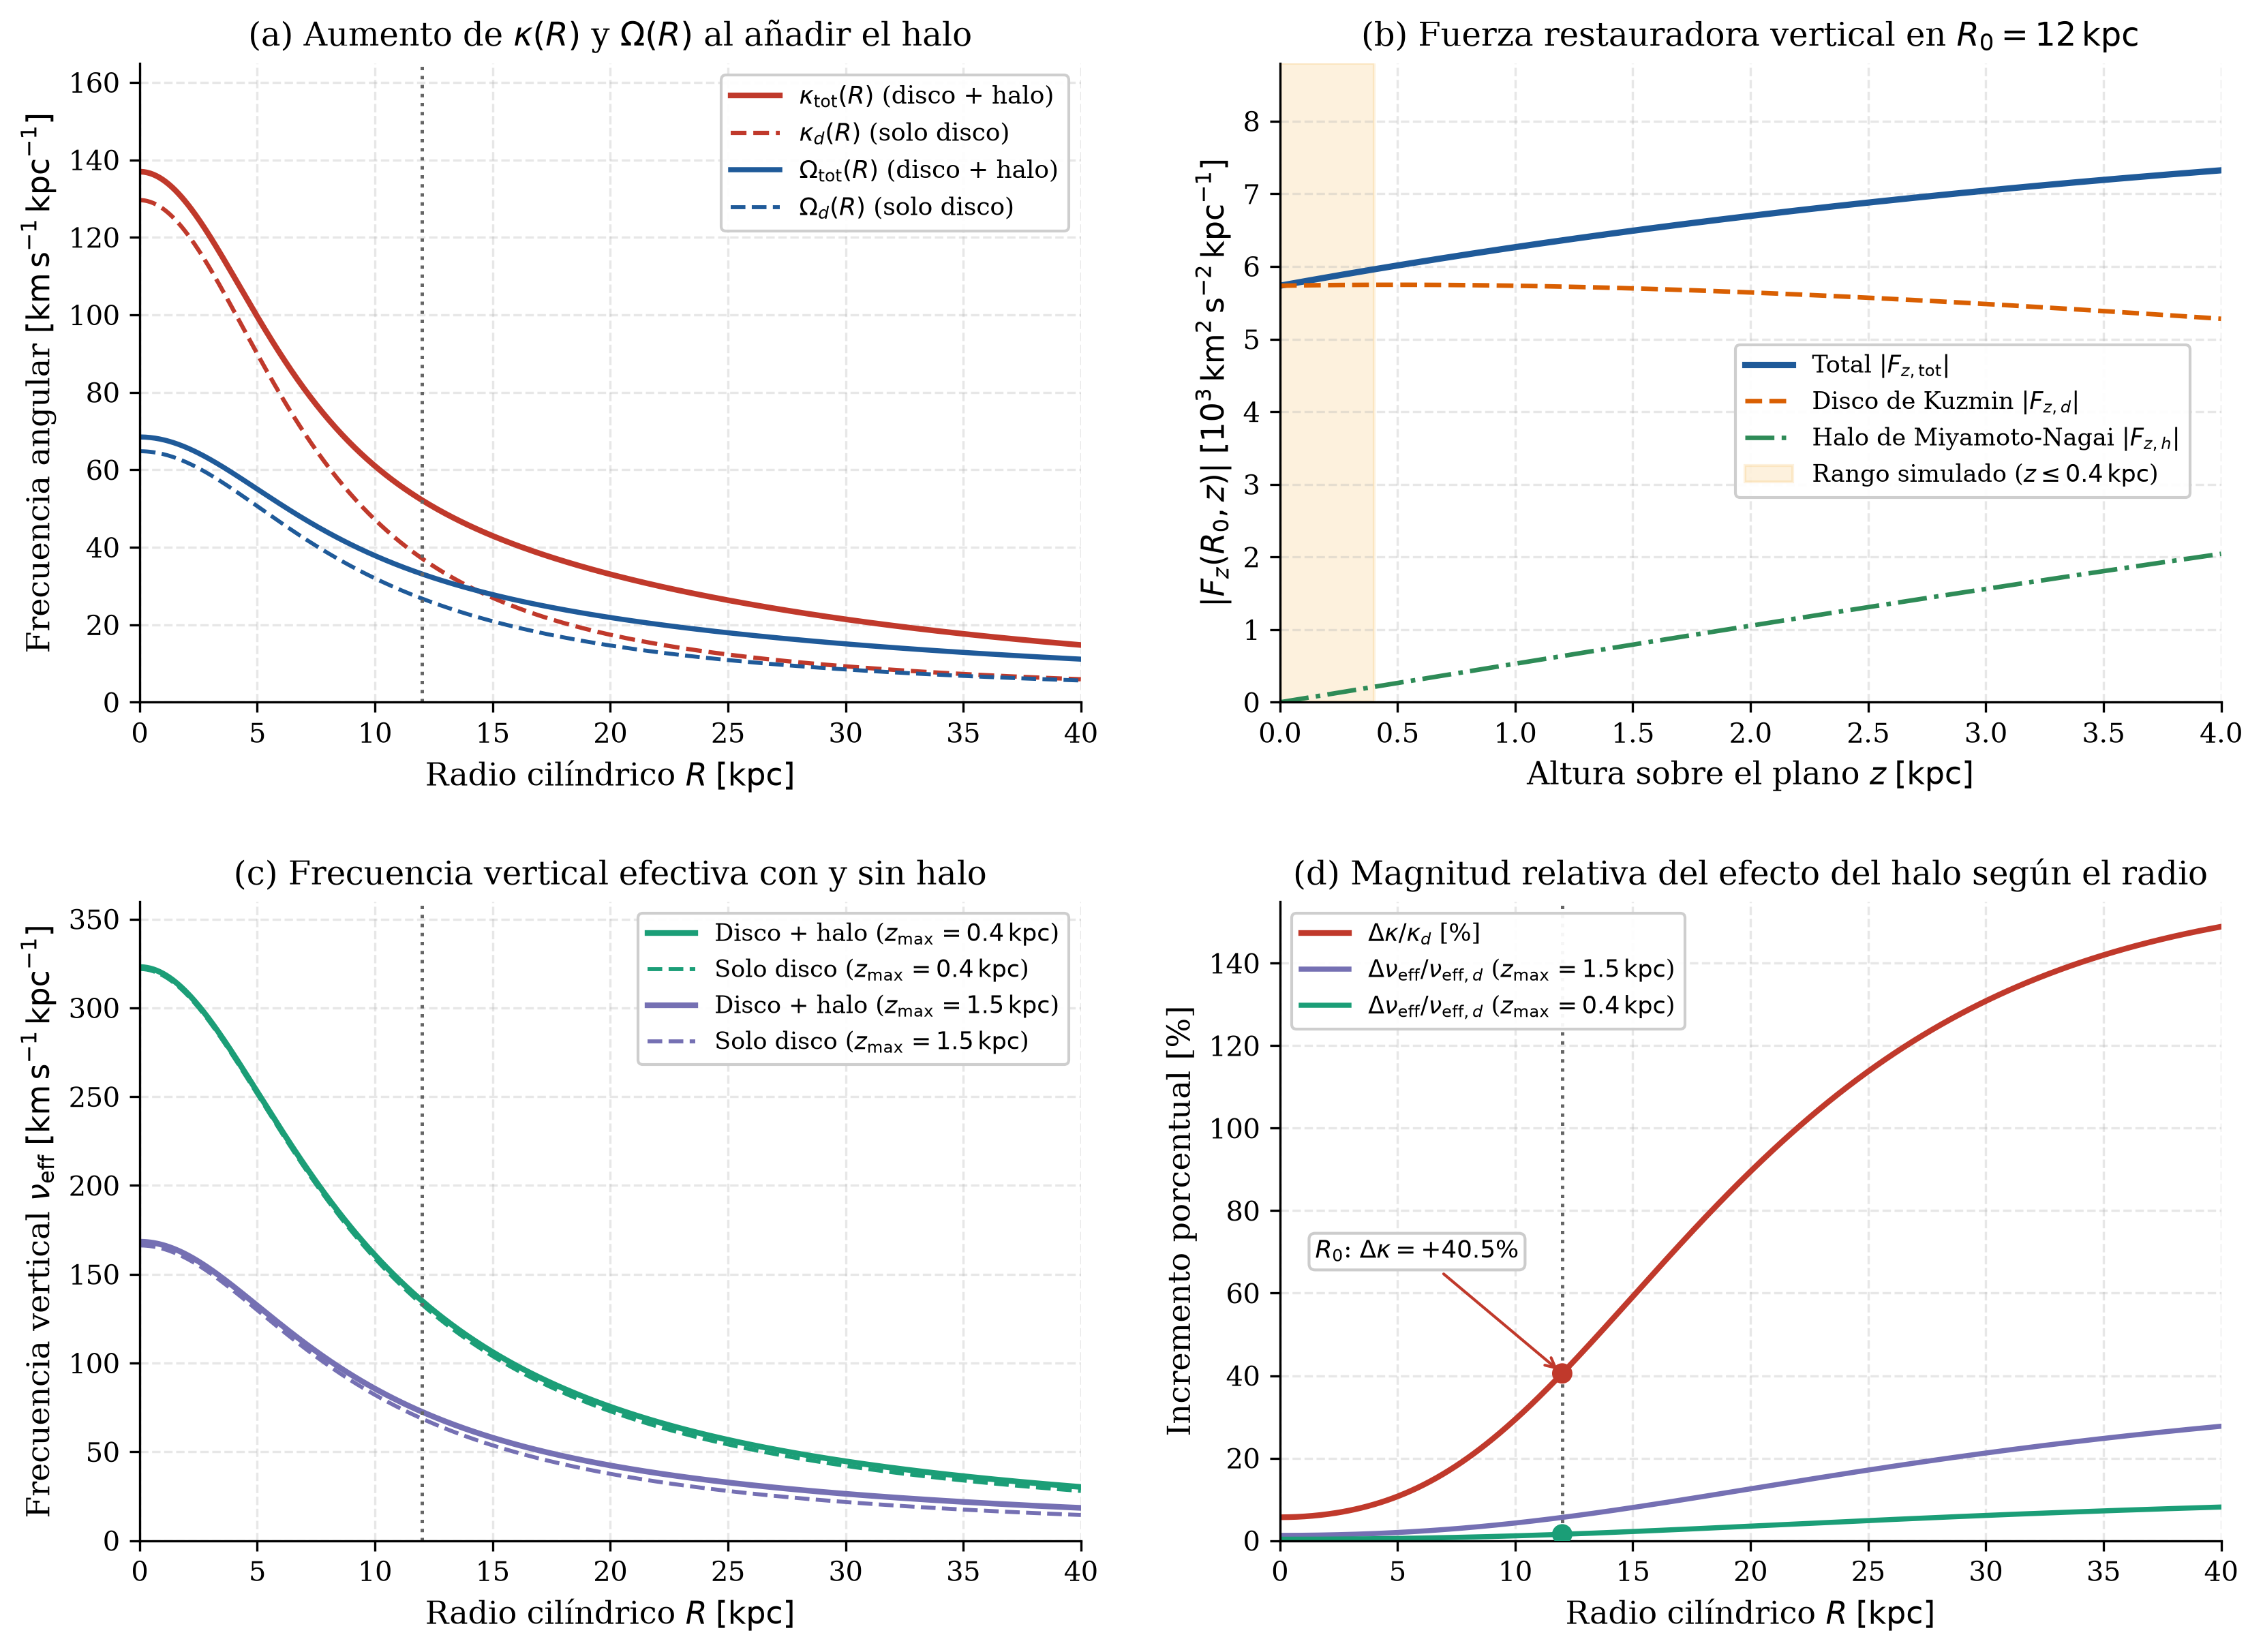
\includegraphics[width=0.98\textwidth]{fig6_frequencies_comparison.png}
    \caption{Predicción analítica del efecto del halo. (a) $\kappa(R)$ y $\Omega(R)$ con y sin halo. (b) Descomposición de la fuerza vertical $|F_z(R_0, z)|$: dominio del disco cerca de $z = 0$ y crecimiento lineal del halo. (c) $\nu_{\mathrm{eff}}(R)$ para dos amplitudes. (d) Incremento porcentual de $\kappa$ y $\nu_{\mathrm{eff}}$ con el radio.}
    \label{fig:freq_comp}
\end{figure}

La Figura~\ref{fig:freq_comp} cuantifica estas predicciones analíticas a lo largo del disco:
\begin{itemize}
    \item \textbf{Aumento fuerte de $\kappa$ (gráficas~a y~d):} en $R_0 = 12\,\mathrm{kpc}$, la frecuencia epicíclica sube de $\kappa_d = 37.13$ a $\kappa_{\mathrm{tot}} = 52.18\,\mathrm{km\,s^{-1}\,kpc^{-1}}$ ($+40.5\%$), y en el disco externo ($R = 25\,\mathrm{kpc}$) el incremento supera $+113\%$.
    \item \textbf{Aumento dependiente de $z$ y $R$ en $\nu_{\mathrm{eff}}$ (gráficas~b, c y~d):} cerca del plano medio en $R_0 = 12\,\mathrm{kpc}$ la densidad superficial del disco domina la fuerza vertical ($|F_{z,d}| \approx 5.7\times 10^3$ inmediatamente sobre $z = 0$), mientras que $|F_{z,h}| \approx \nu_h^2 z$ parte de cero y apenas llega a $\sim 0.2\times 10^3$ en $z = 0.4\,\mathrm{kpc}$ (gráfica~b). Así que en $R_0 = 12\,\mathrm{kpc}$ con $z_{\max} = 0.4\,\mathrm{kpc}$ se predice un aumento modesto ($133.0 \to 135.0\,\mathrm{km\,s^{-1}\,kpc^{-1}}$, $+1.5\%$), que se vuelve mucho más marcado a mayores alturas ($z_{\max} = 1.5\,\mathrm{kpc}$) o en radios externos ($R \gtrsim 25\,\mathrm{kpc}$) donde $\Sigma_K \propto R^{-3}$ decae rápidamente (gráfica~c).
\end{itemize}

\subsection{Simulación en el potencial disco + halo}

Se integra ahora la órbita bajo la aceleración total $\mathbf{a}_{\mathrm{tot}} = \mathbf{a}_K + \mathbf{a}_h = -\nabla\Phi_K - \nabla\Phi_h$ con el mismo integrador Velocity Verlet ($\Delta t = 2.5\times 10^{-5}\,t_u$). En coordenadas cartesianas $(x, y, z)$, sustituyendo $R^2 = x^2 + y^2$ y usando $B \equiv \sqrt{z^2 + b_h^2}$ (con $\mathrm{d}B/\mathrm{d}z = z/B$) y $D_h \equiv \sqrt{x^2 + y^2 + (a_h + B)^2}$, el potencial del halo se escribe:
\begin{equation}
    \Phi_h(x, y, z) = -G M_h\left[x^2 + y^2 + (a_h + B)^2\right]^{-1/2} = -G M_h\,(D_h^2)^{-1/2}.
\end{equation}
Aplicando la regla de la cadena para cualquier coordenada cartesiana $q_i \in \{x, y, z\}$, cada componente de la aceleración del halo $\mathbf{a}_h = -\nabla\Phi_h$ cumple:
\begin{equation}
    a_{h,i} = -\frac{\partial \Phi_h}{\partial q_i}
    = G M_h\left(-\frac{1}{2}\right)(D_h^2)^{-3/2}\,\frac{\partial (D_h^2)}{\partial q_i}
    = -\frac{G M_h}{2 D_h^3}\,\frac{\partial (D_h^2)}{\partial q_i}.
\end{equation}
Evaluando las derivadas parciales de $D_h^2 = x^2 + y^2 + (a_h + B)^2$ respecto a $x$, $y$ y $z$ (usando $\mathrm{d}B/\mathrm{d}z = z/B$), se obtienen las tres componentes exactas:
\begin{align}
    a_{h,x} &= -\frac{G M_h}{2 D_h^3}\,(2x) = -\frac{G M_h\,x}{D_h^3}, \nonumber \\
    a_{h,y} &= -\frac{G M_h}{2 D_h^3}\,(2y) = -\frac{G M_h\,y}{D_h^3}, \\
    a_{h,z} &= -\frac{G M_h}{2 D_h^3}\cdot 2(a_h + B)\,\frac{z}{B} = -\frac{G M_h\,(a_h + B)}{D_h^3}\,\frac{z}{B}. \nonumber
\end{align}

En $R_0 = 12.0\,\mathrm{kpc}$, la nueva velocidad circular de equilibrio es $v_{c,\mathrm{tot}}(R_0) = \sqrt{v_{c,d}^2 + v_{c,h}^2} = 397.48\,\mathrm{km\,s^{-1}}$ y el periodo orbital baja de $229.5$ a $185.5\,\mathrm{Myr}$. Aplicando la misma perturbación relativa de la Sección~2.2 ($\delta v_R = 0.05\,v_{c,\mathrm{tot}}(R_0) \approx 19.87\,\mathrm{km\,s^{-1}}$, $z_0 = 0.40\,\mathrm{kpc}$, $v_z(0) = 0$), las condiciones iniciales quedan en:
\begin{equation}
    \mathbf{r}(0) = (12.0,\; 0,\; 0.40)\,\mathrm{kpc}, \qquad
    \mathbf{v}(0) = (19.8740,\; 397.4802,\; 0)\,\mathrm{km\,s^{-1}}.
\end{equation}
Esta órbita se integra durante $1.0\,t_u$ ($5.3$ periodos orbitales), manteniendo la conservación de integrales en $|\Delta E/E_0| \le 7.0\times 10^{-5}$ y $|\Delta L_z/L_{z,0}| \le 1.4\times 10^{-14}$.

\begin{figure}[H]
    \centering
    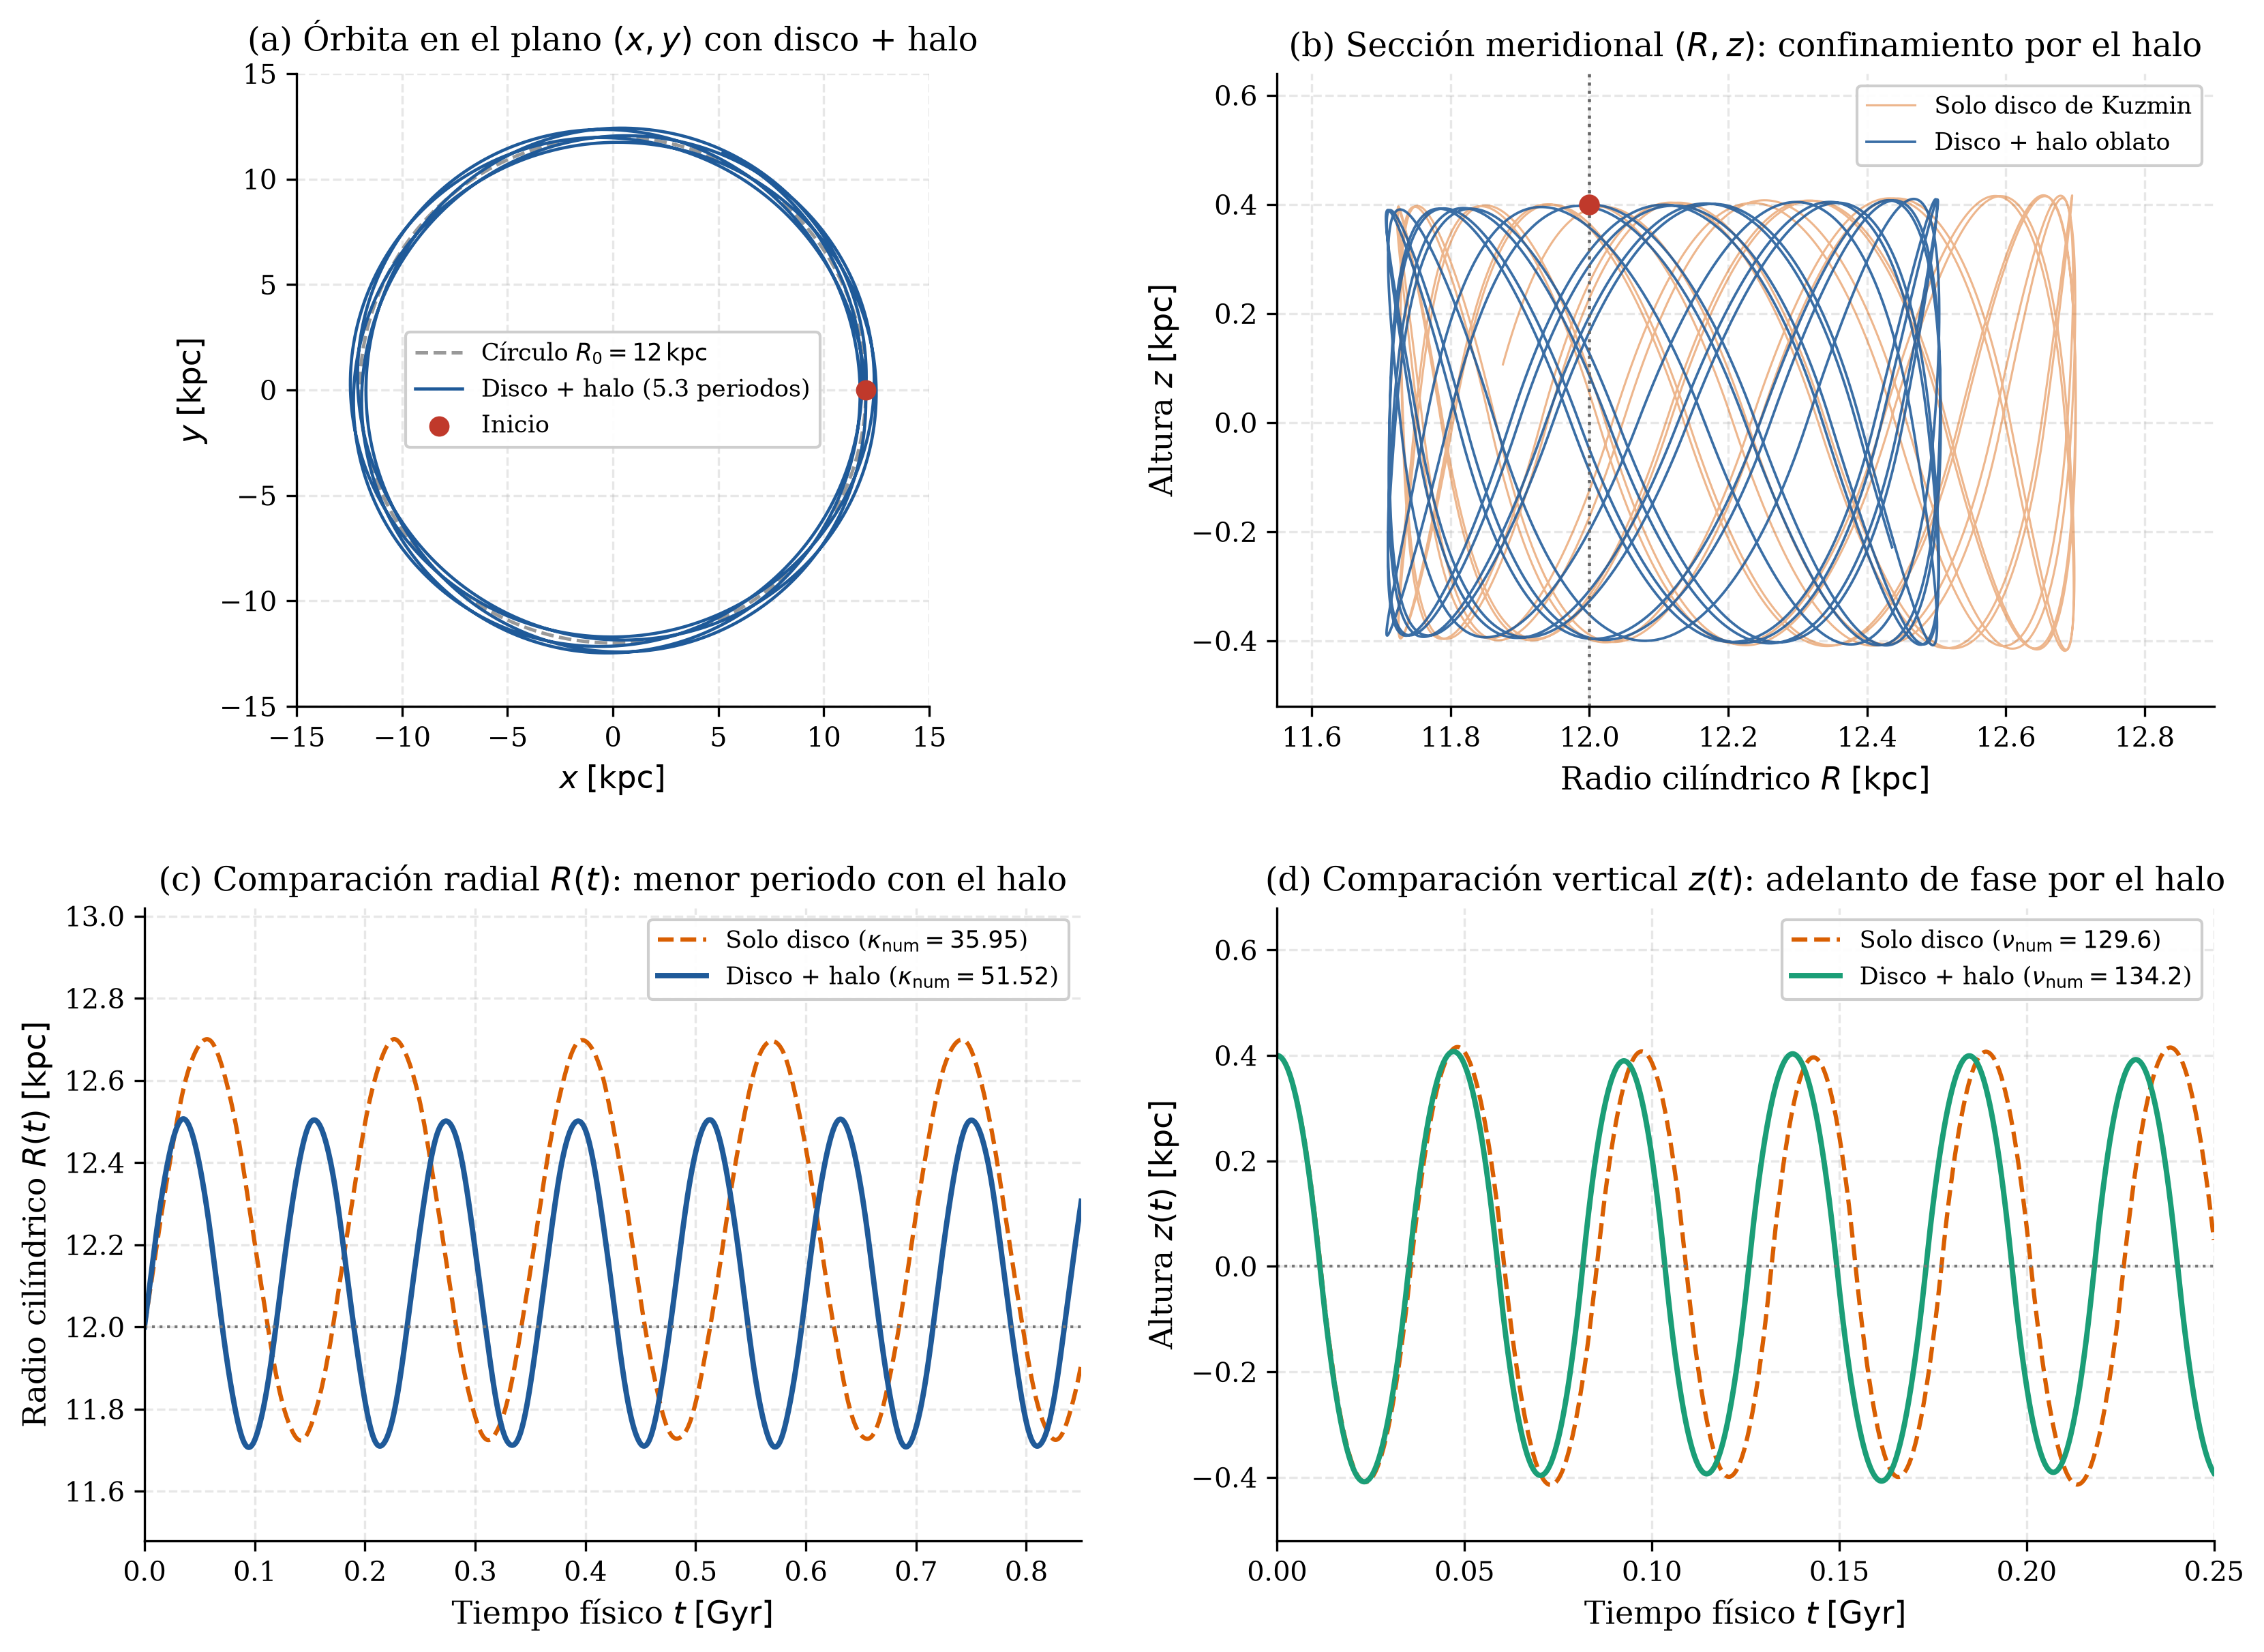
\includegraphics[width=0.98\textwidth]{fig7_disk_halo_orbit.png}
    \caption{Simulación simultánea disco + halo en $R_0 = 12\,\mathrm{kpc}$ comparada con el disco aislado. (a) Órbita no cerrada en el plano $(x,y)$. (b) Sección meridional $(R,z)$. (c) Comparación de $R(t)$ en tiempo físico. (d) Comparación de $z(t)$ mostrando el adelanto de fase por el halo.}
    \label{fig:dh_orbit}
\end{figure}

\begin{table}[H]
    \centering
    \caption{Comparación de frecuencias ($\mathrm{km\,s^{-1}\,kpc^{-1}}$) y periodos ($\mathrm{Myr}$) sin halo y con halo oblato, entre teoría y simulación en $R_0 = 12\,\mathrm{kpc}$ y $R_1 = 25\,\mathrm{kpc}$ ($z_0 = 0.40\,\mathrm{kpc}$).}
    \label{tab:part3}
    \small
    \setlength{\tabcolsep}{6pt}
    \begin{tabular}{@{}lcccc@{}}
        \toprule
        Caso / Magnitud & Disco (teo.) & Disco (num.) & Disco+halo (teo.) & Disco+halo (num.) \\
        \midrule
        \multicolumn{5}{@{}l}{Radio de estudio $R_0 = 12\,\mathrm{kpc}$} \\
        Velocidad circular $v_c\;[\mathrm{km\,s^{-1}}]$ & $321.3$ & --- & $397.5$ & --- \\
        Periodo orbital $T_{\mathrm{orb}}\;[\mathrm{Myr}]$ & $229.5$ & $229.5$ & $185.5$ & $185.5$ \\
        Frecuencia epicíclica $\kappa$ & $37.13$ & $35.95$ & $52.18$ & $51.52$ \\
        Periodo radial $T_\kappa\;[\mathrm{Myr}]$ & $165.5$ & $170.9$ & $117.7$ & $119.2$ \\
        Frecuencia vertical $\nu_{\mathrm{eff}}$ & $133.0$ & $129.6$ & $135.0$ & $134.2$ \\
        Periodo vertical $T_z\;[\mathrm{Myr}]$ & $46.20$ & $47.40$ & $45.50$ & $45.78$ \\
        \midrule
        \multicolumn{5}{@{}l}{Verificación externa $R_1 = 25\,\mathrm{kpc}$} \\
        Frecuencia epicíclica $\kappa$ & $12.33$ & $12.13$ & $26.36$ & $26.28$ \\
        Frecuencia vertical $\nu_{\mathrm{eff}}$ & $54.16$ & $54.10$ & $56.80$ & $57.55$ \\
        \bottomrule
    \end{tabular}
\end{table}

La Figura~\ref{fig:dh_orbit} y la Tabla~\ref{tab:part3} confirman las predicciones:
\begin{itemize}
    \item \textbf{Movimiento radial:} en $0.85\,\mathrm{Gyr}$ la órbita con halo completa cerca de $7$ ciclos radiales frente a menos de $5$ sin halo (gráfica~c). La frecuencia medida sube de $\kappa_{\mathrm{num}} = 35.95$ a $51.52\,\mathrm{km\,s^{-1}\,kpc^{-1}}$, a $1.26\%$ del valor teórico ($52.18$). Además, la amplitud radial disminuye ($0.489 \to 0.400\,\mathrm{kpc}$, gráfica~b) y el radio medio se acerca más a $R_0$ ($12.11$ vs.\ $12.24\,\mathrm{kpc}$), porque el potencial radial del halo varía suavemente en $z$ y reduce el acoplamiento vertical-radial.
    \item \textbf{Movimiento vertical:} en la gráfica~(d) se ve cómo la curva con halo se adelanta progresivamente en fase frente al disco solo. La frecuencia medida sube de $129.6$ a $134.2\,\mathrm{km\,s^{-1}\,kpc^{-1}}$, a $0.61\%$ de la predicción analítica anterior para disco + halo ($135.0$). El incremento numérico ($+3.55\%$) supera levemente al $+1.54\%$ a $R_0$ fijo porque al quedar el radio medio más cerca de $12\,\mathrm{kpc}$ también aumenta un poco el aporte vertical del disco.
    \item \textbf{Verificación en el disco externo ($R_1 = 25\,\mathrm{kpc}$):} repitiendo la simulación en $R_1 = 25\,\mathrm{kpc}$ (Tabla~\ref{tab:part3}), donde el halo domina con mayor fuerza, $\kappa$ aumenta $+117\%$ ($12.13 \to 26.28$) y $\nu_{\mathrm{eff}}$ sube $+6.4\%$ ($54.10 \to 57.55$), en acuerdo con la Figura~\ref{fig:freq_comp}d.
\end{itemize}

% =============================================================================
% Conclusiones
% =============================================================================
\section*{Conclusiones}

En el disco aislado de Kuzmin, la frecuencia de epiciclo radial satisface $1 < \kappa/\Omega < 2$ en todo radio finito (transitando del núcleo armónico $\kappa/\Omega \to 2$ al límite kepleriano $\kappa/\Omega \to 1$), de modo que las órbitas perturbadas son no cerradas. En dirección vertical, el salto discontinuo de la fuerza $\Delta F_z = 4\pi G\Sigma_K(R)$ en $z = 0$ produce una delta de Dirac en $\partial^2\Phi_K/\partial z^2$ y hace divergir la frecuencia armónica estándar (coincidiendo con el límite $b \to 0$ de Miyamoto-Nagai); por tanto, para amplitudes pequeñas la oscilación vertical se describe como un movimiento parabólico a trozos con $\nu_{\mathrm{eff}} \propto \Sigma_K^{1/2} z_{\max}^{-1/2}$ que cumple la jerarquía $\nu_{\mathrm{eff}} > \kappa > \Omega$.

La integración numérica con el esquema de diferencias finitas centradas Velocity Verlet en coordenadas cartesianas reprodujo la órbita de equilibrio en $R_0 = 12\,\mathrm{kpc}$ durante $4$ periodos con errores acotados en $|\Delta E/E_0| \le 2.4\times 10^{-13}$ y $|\Delta L_z/L_{z,0}| \le 1.7\times 10^{-14}$. En la órbita perturbada ($5$ periodos), las frecuencias medidas coinciden con las predicciones analíticas dentro de $2.6\%$--$3.2\%$, mientras que el desplazamiento del radio medio ($12.0 \to 12.24\,\mathrm{kpc}$) y el desfase progresivo tras varios ciclos muestran cómo emergen en la dinámica completa el acoplamiento vertical-radial y la asimetría del pozo efectivo despreciados por la aproximación lineal.

Al incluir el halo oblato de Miyamoto-Nagai achatado a lo largo del eje $z$ ($M_h = 5M_d$, $a_h = 8\,\mathrm{kpc}$, $b_h = 20\,\mathrm{kpc}$, $q_\rho \approx 0.75$), ambas frecuencias aumentan en todo el disco: $\kappa$ crece fuertemente en todos los radios ($+40.5\%$ en $R_0 = 12\,\mathrm{kpc}$ y $+117\%$ en $R_1 = 25\,\mathrm{kpc}$), mientras que $\nu_{\mathrm{eff}}$ aumenta de forma moderada cerca del plano interior (donde domina la fuerza vertical del disco) y se intensifica a mayores alturas y radios externos. La simulación simultánea disco + halo confirmó cuantitativamente estas predicciones (con diferencias de $1.26\%$ en $\kappa$ y $0.61\%$ en $\nu_{\mathrm{eff}}$ en $R_0 = 12\,\mathrm{kpc}$), mostrando además un mayor confinamiento radial y una reducción del acoplamiento entre $R$ y $z$.

% =============================================================================
% Referencias
% =============================================================================
\begin{thebibliography}{3}
    \bibitem{BT2008} Binney, J., \& Tremaine, S. (2008). Galactic Dynamics (2nd ed.). Princeton University Press, Capítulos~2 (\S 2.1, \S 2.3, \S 2.7) y~3 (\S 3.1--\S 3.2, \S 3.4).
    \bibitem{RepoCodigo} Repositorio del trabajo (códigos en Python, figuras y cálculos/ajustes numéricos de parámetros): {\footnotesize\url{https://github.com/andromedalactea/galacticAndExtraGalacticAstrophysics/tree/main/Exam%202}}.
    \bibitem{Gemini2026} Google DeepMind (2026). Gemini [Modelo de lenguaje de gran tamaño]. Utilizado como herramienta de apoyo para conceptualizar el desarrollo, estructurar demostraciones, verificar código y perfeccionar el informe.
\end{thebibliography}

\end{document}
